\documentclass[compress,trans,9pt]{beamer}
% \documentclass[9pt]{beamer}
%\documentclass[compress,9pt,usenames,dvipsnames]{beamer}
% \usepackage[utf8]{inputenc}
% \includeonlyframes{current}
\setbeamercovered{dynamic}
\usepackage{etex}
\usepackage{graphicx,url,psfrag}
\usepackage{tikz}
\usetikzlibrary{
  decorations.pathreplacing,
  calc,
  decorations.fractals,
  through,
  shapes,
  patterns,
  arrows.meta,
  decorations.pathreplacing,
  arrows,
  shapes,
  mindmap
}
\usepackage[center]{subfigure}
\usepackage{enumerate}
\usepackage[makeroom]{cancel}
\usepackage{mathtools}
\usepackage{graphbox}
\usepackage{amssymb}
% \usepackage[showframe]{geometry}
% \usepackage{enumitem}

%
% for warning sign
%
\usepackage{stackengine}
\usepackage{scalerel}
\usepackage{xcolor}
\newcommand\dangersign[1][2ex]{%
  \renewcommand\stacktype{L}%
  \scaleto{\stackon[1.3pt]{\color{red}$\triangle$}{\tiny !}}{#1}%
}
% %  The following is to show codes:
\usepackage{listings}
% \usepackage{color}
\usepackage{colortbl}
\usepackage{dbt}

\definecolor{dkgreen}{rgb}{0,0.6,0}
\definecolor{gray}{rgb}{0.5,0.5,0.5}
\definecolor{mauve}{rgb}{0.58,0,0.82}

% \definecolor{deepblue}{rgb}{0,0,0.5}
% \definecolor{deepred}{rgb}{0.6,0,0}
% \definecolor{deepgreen}{rgb}{0,0.5,0}
% \lstset{
%   language=Python,
%   backgroundcolor=\color{red},  % choose the background color. You must add \usepackage{color}
%   % backgroundcolor=\color{background},  % choose the background color. You must add \usepackage{color}
%   basicstyle=\footnotesize,
%   otherkeywords={self},
%   keywordstyle=\ttb\color{deepblue},
%   emph={MyClass,__init__},
%   emphstyle=\ttb\color{deepred},
%   stringstyle=\color{deepgreen},
%   commentstyle=\color{red},  %%%%%%%%
%   frame=tb,
%   showstringspaces=false
% }
%
% \lstdefinestyle{Python}{
%     language        = Python,
%     basicstyle      = \footnotesize,
%     keywordstyle    = \color{blue},
%     keywordstyle    = [2] \color{red}, % just to check that it works
%     stringstyle     = \color{green},
%     commentstyle    = \color{red}\ttfamily
% }

\lstset{frame=tb,
  language=Java,
  aboveskip=3mm,
  belowskip=3mm,
  showstringspaces=false,
  columns=flexible,
  basicstyle={\small\ttfamily},
  numbers=none,
  numberstyle=\tiny\color{gray},
  keywordstyle=\color{blue},
  commentstyle=\color{dkgreen},
  stringstyle=\color{mauve},
  breaklines=true,
  breakatwhitespace=true,
  tabsize=3
}
\lstset{language=Java}

\lstset{ %
  language=R,                     % the language of the code
  basicstyle=\footnotesize,       % the size of the fonts that are used for the code
  numbers=left,                   % where to put the line-numbers
  numberstyle=\tiny\color{gray},  % the style that is used for the line-numbers
  stepnumber=1,                   % the step between two line-numbers. If it's 1, each line
                                  % will be numbered
  numbersep=5pt,                  % how far the line-numbers are from the code
  backgroundcolor=\color{background},  % choose the background color. You must add \usepackage{color}
  showspaces=false,               % show spaces adding particular underscores
  showstringspaces=false,         % underline spaces within strings
  showtabs=false,                 % show tabs within strings adding particular underscores
  frame=single,                   % adds a frame around the code
  rulecolor=\color{black},        % if not set, the frame-color may be changed on line-breaks within not-black text (e.g. commens (green here))
  tabsize=2,                      % sets default tabsize to 2 spaces
  captionpos=b,                   % sets the caption-position to bottom
  breaklines=true,                % sets automatic line breaking
  breakatwhitespace=false,        % sets if automatic breaks should only happen at whitespace
  title=\lstname,                 % show the filename of files included with \lstinputlisting;
                                  % also try caption instead of title
  keywordstyle=\color{blue},      % keyword style
  commentstyle=\color{dkgreen},   % comment style
  stringstyle=\color{mauve},      % string literal style
  escapeinside={\%*}{*)},         % if you want to add a comment within your code
  morekeywords={*,...}            % if you want to add more keywords to the set
}
% \usepackage[usenames,dvipsnames]{color}
% \lstset{
%   language=Python,                     % the language of the code
%   basicstyle=\footnotesize,       % the size of the fonts that are used for the code
%   numbers=left,                   % where to put the line-numbers
%   numberstyle=\tiny\color{gray},  % the style that is used for the line-numbers
%   stepnumber=1,                   % the step between two line-numbers. If it's 1, each line
%                                   % will be numbered
%   numbersep=5pt,                  % how far the line-numbers are from the code
%   backgroundcolor=\color{background},  % choose the background color. You must add \usepackage{color}
%   showspaces=false,               % show spaces adding particular underscores
%   showstringspaces=false,         % underline spaces within strings
%   showtabs=false,                 % show tabs within strings adding particular underscores
%   frame=single,                   % adds a frame around the code
%   rulecolor=\color{black},        % if not set, the frame-color may be changed on line-breaks within not-black text (e.g. commens (green here))
%   tabsize=2,                      % sets default tabsize to 2 spaces
%   captionpos=b,                   % sets the caption-position to bottom
%   breaklines=true,                % sets automatic line breaking
%   breakatwhitespace=false,        % sets if automatic breaks should only happen at whitespace
%   title=\lstname,                 % show the filename of files included with \lstinputlisting;
%                                   % also try caption instead of title
%   keywordstyle=\ttb\color{blue},      % keyword style
%   commentstyle=\color{dkgreen},   % comment style
%   stringstyle=\color{mauve},      % string literal style
%   escapeinside={\%*}{*)},         % if you want to add a comment within your code
%   morekeywords={*,...}            % if you want to add more keywords to the set
% }

% \usepackage[dvipsnames]{xcolor}
% \newcommand{\Cross}{\mathbin{\tikz [x=1.4ex,y=1.4ex,line width=.2ex] \draw (0,0) -- (1,1) (0,1) -- (1,0);}}%
\newcommand{\Crossme}[1]{\!\!
\tikz [black,x=1.1em,y=1.1em,line width=.4ex]
\draw (-0.5,-0.5) -- (0,0) node {\footnotesize #1} -- (0.5,0.5) (0.5,-0.5) -- (-0.5,0.5);}%
\newcommand{\Checkme}[1]{\!\!
\tikz [x=1.1em,y=1.1em,line width=.4ex]
\draw [black] (0,0.7) -- (0.3,0) --(0.9,1.0) (0.5,0.5) node {\footnotesize #1};}
% \beamerdefaultoverlayspecification{<+-| alert@+>} %(this will show line by line)
\beamerdefaultoverlayspecification{<+->} %(this will show line by

% \usepackage{natbib}
% \input{../myMathSymbols.tex}
% \newcommand{\tlMr}[4]{\:{}^{\hspace{0.2em}#1}_{#2} \hspace{-0.1em}#3_{#4}}

% Smiley face\Smiley{} \Frowny{}
\usepackage{marvosym}
% -------------------------------------------------
%  Set directory for figs
% -------------------------------------------------
\usepackage{grffile}
\graphicspath{{Codes/}}
% -------------------------------------------------
%  Define colors
% -------------------------------------------------
\def\refcolor{cyan}
\newcommand{\myref}[1]{\small {\em #1}}
\def\excolor{brown}
% \usepackage{color}
% \usepackage[dvipsnames]{xcolor}


% % % Define danger sign
\newcommand*{\TakeFourierOrnament}[1]{{%
\fontencoding{U}\fontfamily{futs}\selectfont\char#1}}
\newcommand*{\danger}{\TakeFourierOrnament{66}}


% -------------------------------------------------
%  Define short-hand symbols.
% -------------------------------------------------
\newcommand{\B}{\textbf{B}}
\newcommand{\PP}{\mathbb{P}}
\newcommand{\E}{\mathbb{E}}
\newcommand{\D}{\mathbb{D}}
\newcommand{\W}{\dot{W}}
\newcommand{\ud}{\ensuremath{\mathrm{d}}}
\newcommand{\Ceil}[1]{\left\lceil #1 \right\rceil}
\newcommand{\Floor}[1]{\left\lfloor #1 \right\rfloor}
\newcommand{\sgn}{\text{sgn}}
\newcommand{\Lad}{\text{L}_{\text{ad}}^2}
\newcommand{\SI}[1]{\mathcal{I}\left[#1 \right]}
\newcommand{\SIB}[2]{\mathcal{I}_{#2}\left[#1 \right]}
\newcommand{\Indt}[1]{1_{\left\{#1 \right\}}}
\newcommand{\LadInPrd}[1]{\left\langle #1 \right\rangle_{\text{L}_\text{ad}^2}}
\newcommand{\LadNorm}[1]{\left|\left|  #1 \right|\right|_{\text{L}_\text{ad}^2}}
\newcommand{\Norm}[1]{\left|\left|  #1   \right|\right|}
\newcommand{\Ito}{It\^{o} }
\newcommand{\Itos}{It\^{o}'s }
\newcommand{\spt}[1]{\text{supp}\left(#1\right)}
\newcommand{\InPrd}[1]{\left\langle #1 \right\rangle}
\newcommand{\mr}{\textbf{r}}
\newcommand{\Ei}{\text{Ei}}
\newcommand{\arctanh}{\operatorname{arctanh}}
\newcommand{\ind}[1]{\mathbb{I}_{\left\{ {#1} \right\} }}
\newcommand{\Var}{\text{Var}}
\newcommand{\Cov}{\text{Cov}}
\newcommand{\Corr}{\text{Corr}}

\newcommand{\baseurl}[1]{\footnotesize\url{http://math.emory.edu/~lchen41/teaching/2020_Spring/#1}}


\newcommand*\mystrut[1]{\vrule width0pt height0pt depth#1\relax} % adding vertical space

\DeclareMathOperator{\esssup}{\ensuremath{ess\,sup}}

\newcommand{\steps}[1]{\vskip 0.3cm \textbf{#1}}
\newcommand{\calB}{\mathcal{B}}
\newcommand{\calC}{\mathcal{C}}
\newcommand{\calD}{\mathcal{D}}
\newcommand{\calE}{\mathcal{E}}
\newcommand{\calF}{\mathcal{F}}
\newcommand{\calG}{\mathcal{G}}
\newcommand{\calK}{\mathcal{K}}
\newcommand{\calH}{\mathcal{H}}
\newcommand{\calI}{\mathcal{I}}
\newcommand{\calL}{\mathcal{L}}
\newcommand{\calM}{\mathcal{M}}
\newcommand{\calN}{\mathcal{N}}
\newcommand{\calO}{\mathcal{O}}
\newcommand{\calT}{\mathcal{T}}
\newcommand{\calP}{\mathcal{P}}
\newcommand{\calR}{\mathcal{R}}
\newcommand{\calS}{\mathcal{S}}
\newcommand{\calV}{\mathcal{V}}
\newcommand{\bbC}{\mathbb{C}}
\newcommand{\bbN}{\mathbb{N}}
\newcommand{\bbP}{\mathbb{P}}
\newcommand{\bbZ}{\mathbb{Z}}
\newcommand{\myVec}[1]{\overrightarrow{#1}}
\newcommand{\sincos}{\begin{array}{c} \cos \\ \sin \end{array}\!\!}
\newcommand{\CvBc}[1]{\left\{\:#1\:\right\}}
\newcommand*{\one}{{{\rm 1\mkern-1.5mu}\!{\rm I}}}

\newcommand{\OneFrame}[1]{
\begin{enumerate}\item[#1] \phantom{av} \\[20em]\vfill\phantom{av}\myEnd\end{enumerate}}

\newcommand{\bH}{\ensuremath{\mathrm{H}}}
\newcommand{\Ai}{\ensuremath{\mathrm{Ai}}}

\newcommand{\R}{\mathbb{R}}
\newcommand{\myEnd}{\hfill$\square$}
\newcommand{\myQED}{\hfill\textcolor{lgtblue}{$\blacksquare$}}
\newcommand{\ds}{\displaystyle}
\newcommand{\Shi}{\text{Shi}}
\newcommand{\Chi}{\text{Chi}}
\newcommand{\Erf}{\ensuremath{\mathrm{erf}}}
\newcommand{\Erfc}{\ensuremath{\mathrm{erfc}}}
\newcommand{\He}{\ensuremath{\mathrm{He}}}
\newcommand{\Res}{\ensuremath{\mathrm{Res}}}

\newcommand{\mySeparateLine}{\begin{center}
 \makebox[\linewidth]{\rule{0.6\paperwidth}{0.4pt}}
\end{center}}

\theoremstyle{definition}
% \newtheorem{definition}[theorem]{Definition}
% \newtheorem{hypothesis}[theorem]{Hypothesis}
\newtheorem{assumption}[theorem]{Assumption}

\theoremstyle{plain}
% \newtheorem{theorem}{Theorem}
% \newtheorem{corollary}[theorem]{Corollary}
% \newtheorem{lemma}[theorem]{Lemma}
\newtheorem{proposition}[theorem]{Proposition}

\mode<presentation>
{
%      \usetheme{Warsaw}
%     \usetheme{JuanLesPins}
%  \usetheme{Hannover}
%  \usetheme{Montpellier}
   \useoutertheme{default}
  % or ...

  \setbeamercovered{transparent}
  % or whatever (possibly just delete it)
 \setbeamertemplate{frametitle}{
  \begin{centering}
    \color{blue}
    {\insertframetitle}
    \par
  \end{centering}
  }
}
\usefoottemplate{\hfill \insertframenumber{}}
% \inserttotalframenumber

\usepackage[english]{babel}
% or whatever

% \usepackage[latin1]{inputenc}
% or whatever

\usepackage{times}
\usepackage[T1]{fontenc}
% Or whatever. Note that the encoding and the font should match. If T1
% does not look nice, try deleting the line with the fontenc.

% \DeclareMathOperator{\Lip}{Lip}
\DeclareMathOperator{\lip}{l}
% \DeclareMathOperator{\Vip}{\overline{v}}
% \DeclareMathOperator{\vip}{\underline{v}}
% \DeclareMathOperator{\vv}{v}
% \DeclareMathOperator{\BC}{BC}
% \DeclareMathOperator{\CH}{CD}

\usepackage{pgfpages}
% \setbeameroption{show notes}
% \setbeamertemplate{note page}[plain]
% \setbeameroption{second mode text on second screen=right}
% \setbeameroption{show notes on second screen=right}
%
\title % (optional, use only with long paper titles)
{
Math 362: Mathematical Statistics II
}

% \subtitle
% {Research Plan} % (optional)

\author{Le Chen\\
\url{le.chen@emory.edu}\\
\url{chenle02@gmail.com}\\[2em]
Emory University\\
Atlanta, GA\\[2em]
\textcolor{gray}{\small Last updated on Spring 2021}\\
\textcolor{gray}{\small Last compiled on \today}
}
\institute[Emory University]
{%
\vspace{3em}
% \pgfuseimage{UNLV}
 }
 \vfill
% - Use the \inst command only if there are several affiliations.
% - Keep it simple, no one is interested in your street address.

% \date[Talk at Karlsruhe] % (optional)
% {\today }
 \date[Columbus]{
   2021 Spring\\[1em]
   Creative Commons License\\
   (CC By-NC-SA)
 }

\subject{}
% This is only inserted into the PDF information catalog. Can be left
% out.

% If you have a file called "university-logo-filename.xxx", where xxx
% is a graphic format that can be processed by latex or pdflatex,
% resp., then you can add a logo as follows:

% \pgfdeclareimage[height=0.8cm]{UNLV}{figs/UNLV-186.png}

% Delete this, if you do not want the table of contents to pop up at
% the beginning of each subsection:
% \AtBeginSubsection[]
% {
%   \begin{frame}<beamer>{Outline}
%     \tableofcontents[currentsection,currentsubsection]
%   \end{frame}
% }


% If you wish to uncover everything in a step-wise fashion, uncomment
% the following command:

% \beamerdefaultoverlayspecification{<+->}
% % % % % % % % % % % % % % % % % % %
%  Define a block
% % % % % % % % % % % % % % % % % % %
\newenvironment<>{problock}[1]{%
  \begin{actionenv}#2%
      \def\insertblocktitle{#1}%
      \par%
      \mode<presentation>{%
        \setbeamercolor{block title}{fg=white,bg=olive!95!black}
       \setbeamercolor{block body}{fg=black,bg=olive!25!white}
       \setbeamercolor{itemize item}{fg=white!20!white}
       \setbeamertemplate{itemize item}[triangle]
     }%
      \usebeamertemplate{block begin}}
    {\par\usebeamertemplate{block end}\end{actionenv}}

\newenvironment<>{assblock}[1]{%
  \begin{actionenv}#2%
      \def\insertblocktitle{#1}%
      \par%
      \mode<presentation>{%
        \setbeamercolor{block title}{fg=white,bg=green!50!black}
       \setbeamercolor{block body}{fg=black,bg=green!10}
       \setbeamercolor{itemize item}{fg=green!80!black}
       \setbeamertemplate{itemize item}[triangle]
     }%
      \usebeamertemplate{block begin}}
    {\par\usebeamertemplate{block end}\end{actionenv}}


\newcommand{\mySection}[1]{\section{\S\: #1}\begin{frame}{\myChapter}\tableofcontents[currentsection]\end{frame}}

\AtBeginSection[]
  {
     \begin{frame}<beamer>
     \frametitle{Plan}
     \tableofcontents[currentsection]
     \end{frame}
  }


\begin{document}

\AtBeginSection[]
  {
     \begin{frame}<beamer>
     \frametitle{Plan}
     \tableofcontents[currentsection]
     \end{frame}
  }


%-------------- start slide -------------------------------%{{{
\begin{frame}[noframenumbering]
  \titlepage
\end{frame}
%-------------- end slide -------------------------------%}}}


% \begin{frame}{Outline}
%   \tableofcontents
%   % You might wish to add the option [pausesections]
% \end{frame}


%-------------- start slide -------------------------------%{{{
\begin{frame}
\begin{center}
\huge
 Chapter 5: Estimation
\end{center}
\end{frame}
%-------------- end slide -------------------------------%}}}

\section{\S\: 5.1 Introduction}
\mySection{5.1 Introduction}
%-------------- start slide -------------------------------%{{{ 5.4
\begin{frame}
   % {\S\: 5.1 Introduction}

 {\bf\noindent Motivating example}: Given an unfair coin, or $p$-coin, such that
 \[
 X=
 \begin{cases}
    1 & \text{head with probability $p$},\\
    0 & \text{tail with probability $1-p$,}
 \end{cases}
 \]
 how would you determine the value $p$?
 \vfill
{\bf Solutions:~}
 \begin{enumerate}
  \item You need to try the coin several times, say, three times. What you obtain is ``HHT''.
  \item Draw a conclusion from the experiment you just made.
 \end{enumerate}

 \end{frame}


 \begin{frame}[fragile]

 {\bf\noindent Rationale:~} The choice of the parameter $p$ should be the value that maximizes the probability of the sample.
 \vfill
 \begin{align*}
 \PP(X_1=1,X_2=1,X_3=0) = &
 P(X_1=1)P(X_2=1)P(X_3=0) \\
 = &p^2(1-p).
 \end{align*}
 \vfill
 \pause
\begin{minipage}{0.4\textwidth}
\begin{lstlisting}
# Hello, R.
p <- seq(0,1,0.01)
plot(p,p^2*(1-p),
     type="l",
     col="red")
title("Likelihood")
# add a vertical dotted (4) blue line
abline(v=0.67, col="blue", lty=4)
# add some text
text(0.67,0.01, "2/3")
 \end{lstlisting}
\end{minipage}
\hfill
\begin{minipage}{0.5\textwidth}
 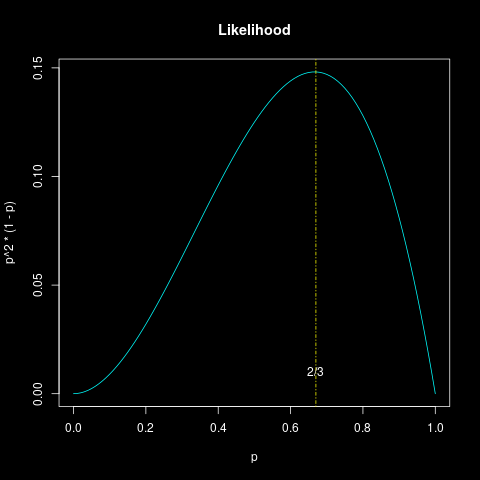
\includegraphics[scale=0.25]{Bernoulli-neg.png}
\end{minipage}
\vfill
Maximize $f(p) = p^2(1-p)$ ....
\end{frame}
%-------------- end slide -------------------------------%}}}
%-------------- start slide -------------------------------%{{{ 5.5
\begin{frame}[fragile]

{\bf A random sample of size $n$ from the population -- Bernoulli$(p)$}: \\[1em]
\begin{itemize}
 \item $X_1, \cdots, X_n$ are i.i.d.\footnote{independent and identically distributed} random variables, each following Bernoulli$(p)$. \\[1em]
 \item Suppose the outcomes of the random sample are: $X_1=k_1,\cdots,X_n=k_n$. \\[1em]
 \item What is your choice of $p$ based on the above random sample?
 \vfill
 \item[]
 \[
 p=\frac{1}{n} \sum_{i=1}^n k_i =: \bar{k}.
 \]
\end{itemize}

\end{frame}
%-------------- end slide -------------------------------%}}}
%-------------- start slide -------------------------------%{{{ 5.6
\begin{frame}

{\bf A random sample of size $n$ from the population with given pdf}: \\[1em]

\begin{itemize}
 \item $X_1, \cdots, X_n$ are i.i.d. random variables, each following the same given pdf.
 \vfill
 \item a {\bf statistic} or an {\bf estimator} is a function of the random sample. \\
 \begin{center}
  \alert{Statistic/Estimator is a random variable!}
 \end{center}
 e.g.,
 \[
 \widehat{p} = \frac{1}{n} \sum_{i=1}^n X_i.
 \]
 \vfill
 \item The outcome of a statistic/estimator is called an {\bf estimate}. e.g.,
 \[
 p_e = \frac{1}{n} \sum_{i=1}^n k_i.
 \]
\end{itemize}
\end{frame}
%-------------- end slide -------------------------------%}}}

\section{\S\: 5.2 Estimating parameters: MLE and MME}
\mySection{5.2 Estimating parameters: MLE and MME}
%-------------- start slide -------------------------------%{{{ 5.10
\begin{frame}
  % {\S\: 5.2 Estimating parameters: MLE and MME}

{\bf\noindent Two methods} for estimating parameters \hfill Corresponding estimator
\vspace{2em}
\begin{enumerate}
 \item Method of maximum likelihood.\hfill MLE \hspace{3em}\phantom{a}
 \vspace{2em}
 \item Method of moments.\hfill MME \hspace{3em}\phantom{a}
\end{enumerate}

% \vf
\end{frame}
%-------------- end slide -------------------------------%}}}
%-------------- start slide -------------------------------%{{{ 5.11
\begin{frame}{Maximum Likelihood Estimation}

{\bf\noindent Definition 5.2.1.~} For a random sample of size $n$ from the
discrete (resp. continuous) population/pdf $p_X(k;\theta)$ (resp.
$f_Y(y;\theta)$), the \textcolor{yellow}{likelihood function}, $L(\theta)$, is the product of
the pdf evaluated at $X_i=k_i$ (resp. $Y_i=y_i$), i.e., \[ L(\theta) =
\prod_{i=1}^n p_X(k_i;\theta) \qquad \bigg(\text{resp.}\: L(\theta) =
\prod_{i=1}^n f_Y(y_i;\theta) \bigg).  \]

\pause \vfill {\bf\noindent Definition 5.2.2.~} Let $L(\theta)$ be as defined
in Definition 5.2.1. If $\theta_e$ is a value of the parameter such that
$L(\theta_e)\ge L(\theta)$ for all possible values of $\theta$, then we call
$\theta_e$ the \textcolor{yellow}{maximum likelihood estimate} for $\theta$.
\end{frame}
%-------------- end slide -------------------------------%}}}
%-------------- start slide -------------------------------%{{{ 5.12
\begin{frame}{Examples for MLE}
Often but not always MLE can be obtained by setting the first derivative equal to zero:\\
\vfill
\begin{enumerate}
 \item[E.g. 1.] Poisson distribution: $p_X(k) = e^{-\lambda}\frac{\lambda^k}{k!}$, $k=0,1,\cdots$.
 \[
 L(\lambda) = \prod_{i=1}^n
e^{-\lambda}\frac{\lambda^{k_i}}{k_i!} = e^{-n\lambda} \lambda^{\sum_{i=1}^k k_i}\left(\prod_{i=1}^n
 k_i!\right)^{-1}.
 \]\pause
 \[
 \ln L(\lambda) = -n\lambda + \left(\sum_{i=1}^{n} k_i\right)\ln \lambda - \ln\left(\prod_{i=1}^{n}k_i!\right).
 \]\pause
 \[
 \frac{\ud }{\ud \lambda} \ln L(\lambda) =  - n + \frac{1}{\lambda}\sum_{i=1}^n k_i.
 \]\pause
 \[
 \frac{\ud }{\ud \lambda} \ln L(\lambda) =0 \quad\Longrightarrow\quad
 \boxed{\lambda_e = \frac{1}{n}\sum_{i=1}^n k_i =: \bar{k}}.
 \]\pause
 \vfill
 {Comment:~} The critical point is indeed global maximum because
 \[
 \frac{\ud^2 }{\ud \lambda^2} \ln L(\lambda) =  - \frac{1}{\lambda^2}\sum_{i=1}^n k_i<0.
 \]
 \end{enumerate}
\end{frame}
%-------------- end slide -------------------------------%}}}
%-------------- start slide -------------------------------%{{{ 5.13
\begin{frame}

The following two cases are related to waiting time: \\[1em]

 \begin{enumerate}
 \item[E.g. 2.] Exponential distribution: $f_Y(y)=\lambda e^{-\lambda y}$ for $y\ge 0$.
 \[
 L(\lambda) = \prod_{i=1}^n
\lambda e^{-\lambda y_i} = \lambda^{n} \exp\left(-\lambda\sum_{i=1}^n y_i\right)
 \]\pause
 \[
 \ln L(\lambda) = n\ln\lambda - \lambda\sum_{i=1}^n y_i.
 \]\pause
 \[
 \frac{\ud }{\ud \lambda} \ln L(\lambda) =   \frac{n}{\lambda} - \sum_{i=1}^n y_i.
 \]\pause
 \[
 \frac{\ud }{\ud \lambda} \ln L(\lambda) =0 \quad\Longrightarrow\quad
 \boxed{\lambda_e = \frac{n}{\sum_{i=1}^n y_i} =: \frac{1}{\bar{y} }}.
 \]
\end{enumerate}

\end{frame}
%-------------- end slide -------------------------------%}}}
%-------------- start slide -------------------------------%{{{ 5.14
\begin{frame}
A random sample of size $n$ from the following population: \\[1em]
 \begin{enumerate}
 \item[E.g. 3.] Gamma distribution: $f_Y(y;\lambda)= \frac{\lambda^r}{\Gamma(r)} y^{r-1} e^{-\lambda y}$ for $y\ge 0$ with $r>1$ known.
 \[
 L(\lambda) = \prod_{i=1}^n
\frac{\lambda^r}{\Gamma(r)} y_i^{r-1} e^{-\lambda y_i} = \lambda^{r \: n} \Gamma(r)^{{-n}} \left(\prod_{i=1}^n y_i^{r-1}\right)\exp\left(-\lambda\sum_{i=1}^n y_i\right)
 \]\pause
 \[
 \ln L(\lambda) = r\: n\ln\lambda -n\ln\Gamma(r)+ \ln\left(\prod_{i=1}^{n}y_i^{r-1}\right)-\lambda\sum_{i=1}^n y_i.
 \]\pause
 \[
 \frac{\ud }{\ud \lambda} \ln L(\lambda) =   \frac{r\: n}{\lambda} -\sum_{i=1}^n y_i.
 \]\pause
 \[
 \frac{\ud }{\ud \lambda} \ln L(\lambda) =0 \quad\Longrightarrow\quad
 \boxed{\lambda_e = \frac{r\: n}{\sum_{i=1}^n y_i} = \frac{r}{\bar{y} }}.
 \]
 \vfill
 Comment:
 \begin{itemize}
  \item When $r=1$, this reduces to the exponential distribution case.
  \item If $r$ is also unknown, it will be much more complicated.\\
  No closed-form solution. One needs numerical solver\footnote{[DW, Example 7.2.25]}.\\
  Try MME instead.
 \end{itemize}
\end{enumerate}
\end{frame}
%-------------- end slide -------------------------------%}}}
%-------------- start slide -------------------------------%{{{ 5.15
\begin{frame}
  A detailed study with data: \\[1em]
 \begin{enumerate}
 \item[E.g. 4.] Geometric distribution: $p_X(k;p)=  (1-p)^{k-1} p$, $k=1,2,\cdots$.
 \[
 L(p) = \prod_{i=1}^n (1-p)^{k_i-1} p
 = (1-p)^{-n+ \sum_{i=1}^k k_i }p^n.
 \]\pause
 \[
 \ln L(p) = \left(-n+\sum_{i=1}^n k_i\right) \ln(1-p) + n\ln p.
 \]\pause
 \[
 \frac{\ud }{\ud p} \ln L(p) =  -\frac{-n+\sum_{i=1}^n k_i}{1-p} +\frac{n}{p}.
 \]\pause
 \[
 \frac{\ud }{\ud p} \ln L(p) =0 \quad\Longrightarrow\quad
 \boxed{p_e= \frac{n}{\sum_{i=1}^n k_i} = \frac{1}{\bar{k} }}.
 \]\pause
\vfill
Comment: Its cousin distribution, the negative binomial distribution can be worked out similarly (See Ex 5.2.14).
 \end{enumerate}
\end{frame}
%-------------- end slide -------------------------------%}}}
%-------------- start slide -------------------------------%{{{ 5.16
\begin{frame}
	\begin{center}
		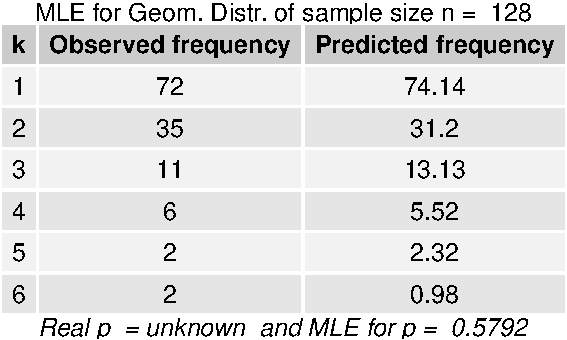
\includegraphics[scale=0.7]{Geometric.pdf}
	\end{center}
\end{frame}
%-------------- end slide -------------------------------%}}}
%-------------- start slide -------------------------------%{{{ 5.17
\begin{frame}[fragile]

 \begin{lstlisting}
# The example from the book.
library(pracma) # Load the library "Practical Numerical Math Functions"
k<-c(72, 35, 11, 6, 2, 2) # observed freq.
a=1:6
pe=sum(k)/dot(k,a) # MLE for p.
f=a
for (i in 1:6) {
  f[i] = round((1-pe)^(i-1) * pe * sum(k),2)
}
# Initialize the table
d <-matrix(1:18, nrow = 6, ncol = 3)
# Now adding the column names
colnames(d) <- c("k",
                 "Observed freq.",
                 "Predicted freq.")
d[1:6,1]<-a
d[1:6,2]<-k
d[1:6,3]<-f
grid.table(d) # Show the table
PlotResults("unknown", pe, d, "Geometric.pdf") # Output the results using a user defined function
\end{lstlisting}
\end{frame}
%-------------- end slide -------------------------------%}}}
%-------------- start slide -------------------------------%{{{ 5.18
\begin{frame}
	\begin{center}
		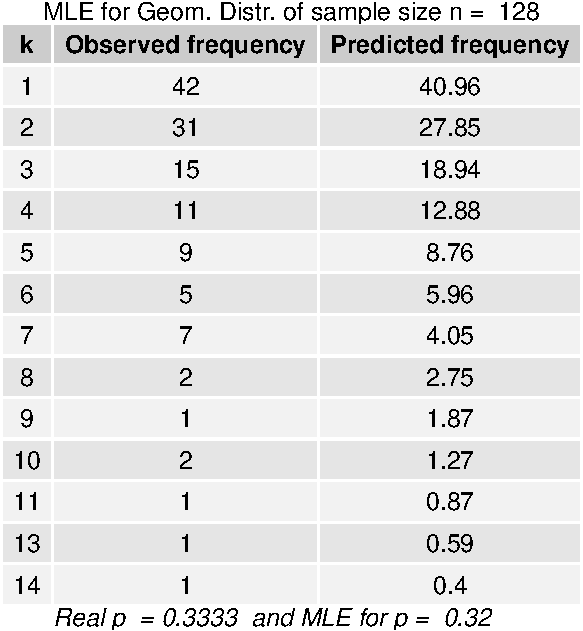
\includegraphics[scale=0.7]{Geometric2.pdf}
	\end{center}
\end{frame}
%-------------- end slide -------------------------------%}}}
%-------------- start slide -------------------------------%{{{ 5.19
\begin{frame}[fragile]

 \begin{lstlisting}
# Now let's generate random samples from a Geometric distribution with p=1/3 with the same size of the sample.
p = 1/3
n = 128
gdata<-rgeom(n, p)+1 # Generate random samples
g<- table(gdata) # Count frequency of your data.
g<- t(rbind(as.numeric(rownames(g)), g)) # Transpose and combine two columns.
pe=n/dot(g[,1],g[,2]) # MLE for p.
f <- g[,1] # Initialize f
for (i in 1:nrow(g)) {
  f[i] = round((1-pe)^(i-1) * pe * n,2)
} # Compute the expected frequency
g<-cbind(g,f) # Add one columns to your matrix.
colnames(g) <- c("k",
                 "Observed freq.",
                 "Predicted freq.") # Specify the column names.
d_df <- as.data.frame(d) # One can use data frame to store data
d_df # Show data on your terminal
PlotResults(p, pe, g, "Geometric2.pdf") # Output the results using a user defined function
 \end{lstlisting}

\end{frame}
%-------------- end slide -------------------------------%}}}
%-------------- start slide -------------------------------%{{{ 5.20
\begin{frame}
	\begin{center}
		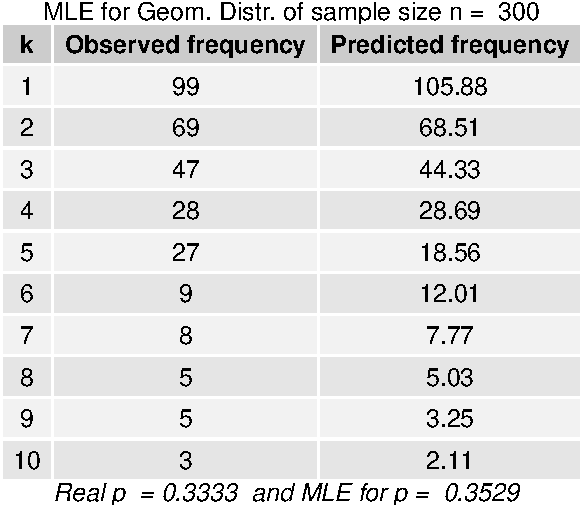
\includegraphics[scale=0.7]{Geometric3.pdf}
	\end{center}
\end{frame}
%-------------- end slide -------------------------------%}}}
%-------------- start slide -------------------------------%{{{ 5.21
\begin{frame}


In case we have several parameters:
\vfill

 \begin{enumerate}
 \item[E.g. 5.] Normal distribution: $f_Y(y;\mu,\sigma^2)= \frac{1}{\sqrt{2\pi} \sigma} e^{-\frac{(y-\mu)^2}{2\sigma^2}}$, $y\in\R$.
 \[
 L(\mu,\sigma^2) = \prod_{i=1}^n \frac{1}{\sqrt{2\pi} \sigma} e^{-\frac{(y_i-\mu)^2}{2\sigma^2}}
 = (2\pi\sigma^2)^{-n/2} \exp\left(-\frac{1}{2\sigma^2}\sum_{i=1}^n(y_i-\mu)^2 \right)
 \]\pause
 \[
 \ln L(\mu,\sigma^2) = -\frac{n}{2}\ln(2\pi\sigma^2) -\frac{1}{2\sigma^2}\sum_{i=1}^n (y_i-\mu)^2.
 \]\pause
 \[
 \begin{cases}
  \displaystyle \frac{\partial }{\partial \mu} \ln L(\mu,\sigma^2) = \frac{1}{\sigma^2}\sum_{i=1}^n
(y_i-\mu) \\
\displaystyle  \frac{\partial }{\partial \sigma^2} \ln L(\mu,\sigma^2) = -\frac{n}{2\sigma^2}+\frac{1}{2\sigma^4}\sum_{i=1}^n(y_i-\mu)^2
\end{cases}
 \]\pause
 \[
 \begin{cases}
  \displaystyle \frac{\partial }{\partial \mu} \ln L(\mu,\sigma^2) = 0\\
\displaystyle  \frac{\partial }{\partial \sigma^2} \ln L(\mu,\sigma^2) =0
\end{cases}
\quad\Longrightarrow\quad
\boxed{\begin{cases}
 \displaystyle \mu_e=\bar{y}\\
 \displaystyle  \sigma_e^2=\frac{1}{n}\sum_{i=1}^n(y_i-\bar{y})^2
\end{cases}}
 \]
\end{enumerate}

\end{frame}
%-------------- end slide -------------------------------%}}}
%-------------- start slide -------------------------------%{{{ 5.22
\begin{frame}
In case when the parameters determine the support of the density:\\
(Non regular case)
\vfill

 \begin{enumerate}
 \item[E.g. 6.] Uniform distribution on $[a,b]$ with $a<b$: $f_Y(y;a,b)=\frac{1}{b-a}$ if $y\in [a,b]$.
 \[
 L(a,b) =
 \begin{cases}
  \prod_{i=1}^n \frac{1}{b-a} =\frac{1}{(b-a)^n}  & \text{if $a\le y_1,\cdots,y_n\le b$,}\\
  0  & \text{otherwise.}
 \end{cases}
 \]\pause
 $L(a,b)$ is monotone increasing in $a$ and decreasing in $b$. Hence, in order to maximize $L(a,b)$,
 one needs to choose
 \[
  a_e=y_{min} \quad\text{and}\quad b_e=y_{max}.
 \]\pause
 \vfill
  \item[E.g. 7.] $f_Y(y;\theta) = \frac{2y}{\theta^2}$ for $y\in [0,\theta]$.
  \[
 L(\theta) =
 \begin{cases}
  \prod_{i=1}^n \frac{2y_i}{\theta^2} =2^n \theta^{-2n}\prod_{i=1}^n y_i  & \text{if $0\le y_1,\cdots,y_n\le \theta$,}\\
  0  & \text{otherwise.}
 \end{cases}
  \]\pause
  \[
  \Downarrow
  \]
  \[
  \theta_e = y_{max}.
  \]
  \end{enumerate}
\end{frame}
%-------------- end slide -------------------------------%}}}
%-------------- start slide -------------------------------%{{{ 5.23
\begin{frame}[fragile]
In case of discrete parameter:
\vfill
\begin{enumerate}
 \item[E.g. 8.] {\bf Wildlife sampling.}  Capture-tag-recapture.... In the history, $a$ tags have been put.
 In order to estimate the population size $N$, one randomly captures $n$ animals, and there are $k$ tagged. Find the MLE for $N$.\\
 \vfill
 {\bf Sol.}
 The population follows hypergeometric distr.: $p_X(k;N)=\frac{{a\choose k}{N-a\choose n-k}}{{N\choose n}}$.\\ \pause
 \[
 L(N) = \frac{{a\choose k}{N-a\choose n-k}}{{N\choose n}}
 \]\pause
 How to maximize $L(N)$? \\ \pause
 \begin{minipage}{0.4\textwidth}
 \begin{lstlisting}
> a=10
> k=5
> n=20
> N=seq(a,a+100)
> p=choose(a,k)*choose(N-a,n-k)/choose(N,n)
> plot(N,p,type = "p")
> print(paste("The MLE is", n*a/k))
[1] "The MLE is 40"
 \end{lstlisting}
 \end{minipage}
 \quad
 \begin{minipage}{ 0.45\textwidth}
	 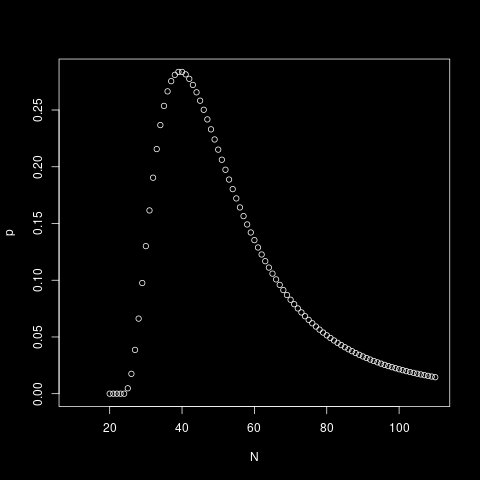
\includegraphics[scale=0.25]{Wildlife-neg.png}
 \end{minipage}
\end{enumerate}
\end{frame}
%-------------- end slide -------------------------------%}}}
%-------------- start slide -------------------------------%{{{ 5.24
\begin{frame}
	\begin{enumerate}
		\item[] The graph suggests to sudty the following quantity:
			\vfill
 \[
 r(N) := \frac{L(N)}{L(N-1)} =\frac{N-n}{N} \times \frac{N-a}{N-a-n+k}
 \]
 \vfill \pause
 \[
 r(N)<1 \quad\Longleftrightarrow \quad na<Nk \quad \text{i.e., $N>\frac{na}{k}$}
 \]\pause
 \vfill
 \[
\boxed{ N_e = \mathop{\arg\max} \left\{ L(N): N = \Floor{\frac{na}{k}}, \Ceil{\frac{na}{k}} \right\}}.
 \]
 \myEnd
	\end{enumerate}
\end{frame}
%-------------- end slide -------------------------------%}}}
%-------------- start slide -------------------------------%{{{ 5.25
\begin{frame}{Method of Moments Estimation}

 {\bf Rationale:~} The population moments should be close to the sample moments, i.e.,
 \[
\E(Y^k) \approx \frac{1}{n}\sum_{i=1}^ny_i^k , \quad k=1,2,3,\cdots.
 \]

 \vfill
{\bf\noindent Definition 5.2.3.~}  For a random sample of size $n$ from the discrete (resp. continuous) population/pdf $p_X(k;\theta_1,\cdots,\theta_s)$ (resp. $f_Y(y;\theta_1,\cdots,\theta_s)$), solutions to
\[
\begin{cases}
 \E(Y)  = \frac{1}{n}\sum_{i=1}^n y_i \\
 \qquad \vdots\\
 \E(Y^s)  = \frac{1}{n}\sum_{i=1}^n y_i^s \\
\end{cases}
\]
which are denoted by $\theta_{1e},\cdots, \theta_{se}$,
are called the {\bf method of moments estimates} of $\theta_1,\cdots, \theta_s$.
\end{frame}
%-------------- end slide -------------------------------%}}}
%-------------- start slide -------------------------------%{{{ 5.26
\begin{frame}{Examples for MME}
 MME is often the same as MLE:\\
 \vfill
 \begin{enumerate}
  \item[E.g. 1.] Normal distribution: $f_Y(y;\mu,\sigma^2)= \frac{1}{\sqrt{2\pi} \sigma} e^{-\frac{(y-\mu)^2}{2\sigma^2}}$, $y\in\R$.
  \vfill
  \[
  \begin{cases}
   \displaystyle
   \mu  = \E(Y) = \frac{1}{n} \sum_{i=1}^n y_i = \bar{y}\\
   \displaystyle
   \sigma^2 + \mu^2  = \E(Y^2) = \frac{1}{n} \sum_{i=1}^n y_i^2 \\
  \end{cases}
  \quad\Rightarrow\quad
  \begin{cases}
   \displaystyle
   \mu_e  =  \bar{y}\\
   \displaystyle
   \sigma_e^2 = \frac{1}{n} \sum_{i=1}^n y_i^2 -\mu_e^2 \\
   \phantom{\sigma_e^2 }= \frac{1}{n}\sum_{i=1}^n\left(y_i-\bar{y}\right)^2
  \end{cases}
  \]
\vfill
More examples when MLE coincides with MME: Poisson, Exponential, Geometric.
\end{enumerate}
\end{frame}
%-------------- end slide -------------------------------%}}}
%-------------- start slide -------------------------------%{{{ 5.27
\begin{frame}
MME is often much more tractable than MLE:\\
 \vfill
 \begin{enumerate}
  \item[E.g. 2.] Gamma distribution\footnote{Check Theorem 4.6.3 on p. 269 for mean and variance}: $f_Y(y;r, \lambda)= \frac{\lambda^r}{\Gamma(r)} y^{r-1} e^{-\lambda y}$ for $y\ge 0$.
  \[
  \begin{cases}
   \displaystyle
   \frac{r}{\lambda} = \E(Y) = \frac{1}{n} \sum_{i=1}^n y_i = \bar{y}\\
   \displaystyle
   \frac{r}{\lambda^2} + \frac{r^2}{\lambda^2}  = \E(Y^2) = \frac{1}{n} \sum_{i=1}^n y_i^2 \\
  \end{cases}
  \quad\Rightarrow\quad
  \begin{cases}
   \displaystyle
   r_e = \frac{\bar{y}^2}{\hat{\sigma}^2} \\[1em]
   \displaystyle
   \lambda_e = \frac{\bar{y}}{\hat{\sigma}^2} = \frac{r_e}{\bar{y}}
  \end{cases}
  \]
  where $\bar{y}$ is the sample mean and $\hat{\sigma}^2$ is the sample variance: $\hat{\sigma}^2:= \frac{1}{n}\sum_{i=1}^n(y_i-\bar{y})^2$.
  \vfill
 Comments: MME for $\lambda$ is consistent with MLE when $r$ is known.
 \end{enumerate}
 \end{frame}
%-------------- end slide -------------------------------%}}}
%-------------- start slide -------------------------------%{{{ 5.28
\begin{frame}
  Another tractable example for MME, while less tractable for MLE: \\
  \vfill
  \begin{enumerate}
  \item[E.g. 3.] Neg. binomial distribution: $p_X(k;p,r)={k+r-1\choose k}(1-p)^k p^r$, $k=0,1,\cdots$.
 \[
  \begin{cases}
   \displaystyle
   \frac{r(1-p)}{p} =\E(X) = \bar{k}\\
   \displaystyle
   \frac{r(1-p)}{p^2}= \text{Var}(X) =  \hat{\sigma}^2
  \end{cases}
  \quad\Rightarrow\quad
  \begin{cases}
   \displaystyle
   p_e = \frac{\bar{k}}{\hat{\sigma}^2} \\[1em]
   \displaystyle
   r_e = \frac{\bar{k}^2}{\hat{\sigma}^2-\bar{k}}
  \end{cases}
  \]
 \end{enumerate}

\end{frame}
%-------------- end slide -------------------------------%}}}
%-------------- start slide -------------------------------%{{{ 5.29
\begin{frame}
\begin{center}
 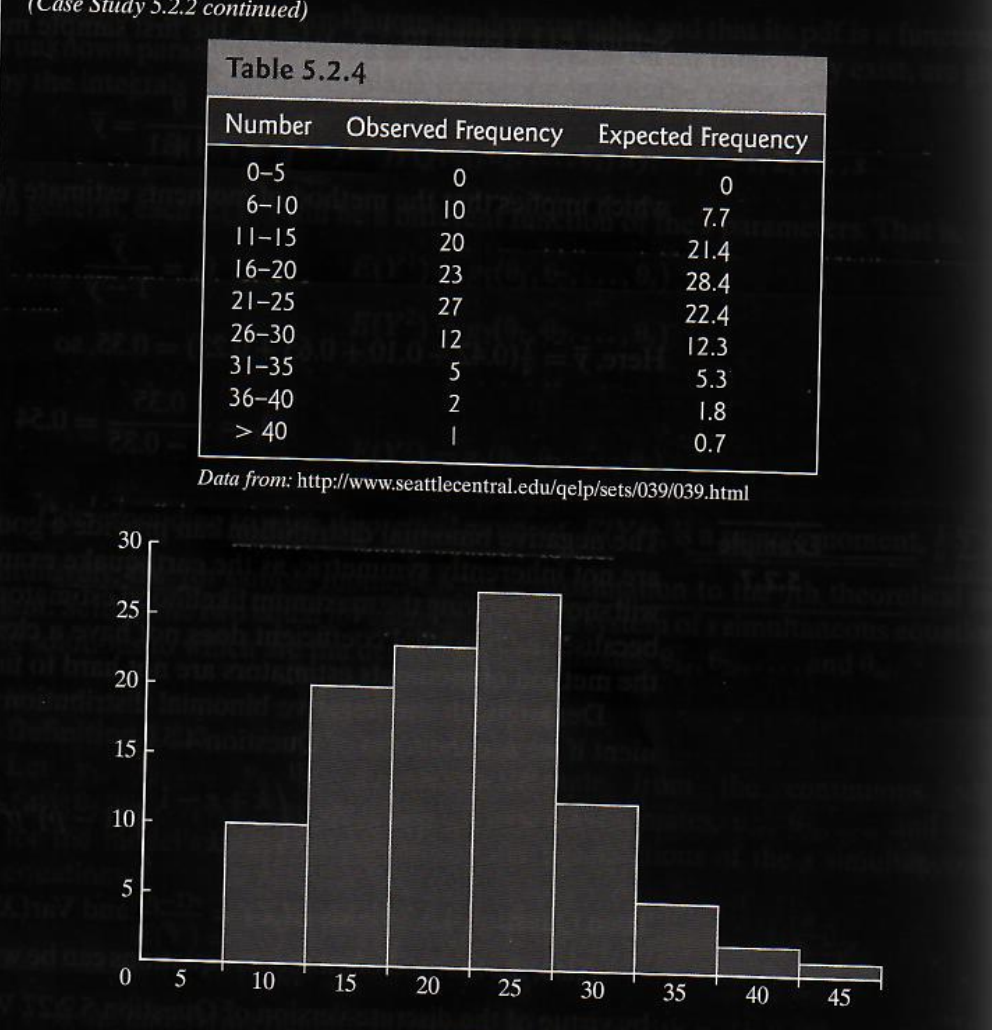
\includegraphics[scale=0.22]{figure-5-2-2-neg.png}\\
 {$r_e=12.74$ and $p_e=0.391$.}
\end{center}
\end{frame}
%-------------- end slide -------------------------------%}}}
%-------------- start slide -------------------------------%{{{ 5.30
\begin{frame}
  \begin{enumerate}
  \item[E.g. 4.] $f_Y(y;\theta) = \frac{2y}{\theta^2}$ for $y\in [0,\theta]$.\\[2em]
  \[
  \overline{y} = \E[Y] = \int_0^\theta \frac{2y^2}{\theta^2}\ud y = \frac{2}{3} \frac{y^3}{\theta^2}\bigg|_{y=0}^{y=\theta} = \frac{2}{3}\theta.
  \]
  \[
  \Downarrow
  \]
  \[
  \boxed{\theta_e = \frac{3}{2}\overline{y}.}
  \]
 \end{enumerate}

\end{frame}
%-------------- end slide -------------------------------%}}}

\section{\S\: 5.3 Interval Estimation}
% \mySection{5.3 Interval Estimation}
%-------------- start slide -------------------------------%{{{ 5.34
\begin{frame}{\S\: 5.3 Interval Estimation}

 {\bf Rationale.~} Point estimate doesn't provide precision information. \\[1em]
  By using the variance of the estimator, one can construct \underline{an interval} such that with a \underline{\underline{high probability}} that interval will contain the unknown parameter.
 \\[1em]
 \begin{itemize}
  \item The \underline{interval} is called {\bf confidence interval}.\\[1em]
  \item The \underline{\underline{high probability}} is {\bf confidence level}.
 \end{itemize}
 \end{frame}

 \begin{frame}
\begin{enumerate}
 \item[E.g. 1.] A random sample of size $4$, ($Y_1 = 6.5$, $Y_2=9.2$, $Y_3=9.9$, $Y_4=12.4$),  from a normal population:
 \[
 f_Y(y;\mu) = \frac{1}{\sqrt{2\pi} \: 0.8} e^{-\frac{1}{2}\left(\frac{y-\mu}{0.8}\right)^2}.
 \]
 Both MLE and MME give $\mu_e = \bar{y} = \frac{1}{4}(6.5+9.2+9.9+12.4)=9.5$.
 The estimator $\widehat\mu=\overline{Y}$ follows normal distribution. \\[3em]
 Construct $95\%$-confidence interval for $\mu$ ...
\end{enumerate}
\end{frame}
%-------------- end slide -------------------------------%}}}
%-------------- start slide -------------------------------%{{{ 5.35
\begin{frame}
\begin{quotation}
  ``The parameter is an unknown constant and no probability statement concerning its value may be made." \\[1em]
--Jerzy Neyman, original developer of confidence intervals.
\end{quotation}
 \vfill
 \begin{center}
  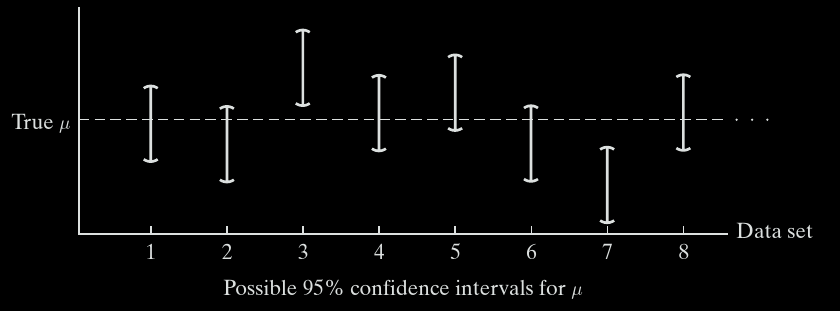
\includegraphics[scale=0.35]{Figure-5-3-2-neg.png}
\end{center}
\end{frame}
%-------------- end slide -------------------------------%}}}
%-------------- start slide -------------------------------%{{{ 5.36
\begin{frame}
  In general, for a normal population with $\sigma$ known, the {\bf $100(1-\alpha)\%$ confidence interval} for $\mu$ is
  \[
  \left(\bar{y} - z_{\alpha/2}\frac{\sigma}{\sqrt{n}}, \bar{y} + z_{\alpha/2}\frac{\sigma}{\sqrt{n}}\right)
  \]
\vfill
\pause
Comment: There are many variations
\begin{enumerate}
 \item One-sided interval such as
 \[
 \left(\bar{y} - z_{\alpha}\frac{\sigma}{\sqrt{n}}, \bar{y} \right)
 \quad\text{or}\quad
 \left(\bar{y}, \bar{y} + z_{\alpha}\frac{\sigma}{\sqrt{n}}\right)
 \]
 \item $\sigma$ is unknown and sample size is small: \hfill $z$-score $\rightarrow$ $t$-score
 \item $\sigma$ is unknown and sample size is large: \hfill $z$-score by CLT\\[1em]
 \item Non-Gaussian population but sample size is large: \hfill  $z$-score by CLT
\end{enumerate}
\end{frame}
%-------------- end slide -------------------------------%}}}
%-------------- start slide -------------------------------%{{{ 5.37
\begin{frame}

{\bf Theorem.~} Let $k$ be the number of successes in $n$ independent trials, where $n$ is large and
$p = \PP(success)$ is unknown. An approximate $100(1-\alpha)\%$ confidence interval for $p$ is
the set of numbers
 \[
 \left(\frac{k}{n}-z_{\alpha/2} \sqrt{\frac{(k/n)(1-k/n)}{n}},\:\frac{k}{n}+z_{\alpha/2} \sqrt{\frac{(k/n)(1-k/n)}{n}}\right).
 \]
\pause
\vfill
Proof: It follows the following facts:
\begin{itemize}
  \item $X\sim$binomial$(n,p)$ iff $X=Y_1+\cdots+Y_n$, while $Y_i$ are i.i.d. Bernoulli$(p)$:
  \begin{align*}
    \E[Y_i] = p\quad\text{and}\quad \Var(Y_i)=p(1-p).
  \end{align*}
  \item {\bf Central Limit Theorem}: Let $W_1, W_2,\cdots, W_n$ be an sequence of i.i.d. random variables, whose distribution has mean $\mu$ and variance  $\sigma^2$, then
    \begin{align*}
      \frac{\sum_{i=1}^n W_i - n\mu}{\sqrt{n\sigma^2 }} \quad \text{{\it approximately} follows}\quad N(0,1),\quad \text{when $n$ is large.}
    \end{align*}
\end{itemize}
\end{frame}
%-------------- end slide -------------------------------%}}}
%-------------- start slide -------------------------------%{{{ 1
\begin{frame}[fragile]
\begin{itemize}
  \item When the sample size $n$ is large, by the central limit theorem,
    \begin{align*}
      \frac{\sum_{i=1}^n Y_i - np}{\sqrt{np(1-p)}}
      \quad \stackrel{\text{ap.}}{\sim}\quad  N(0,1)
    \end{align*}
    \pause
    \[||\hspace{5em}\phantom{a}\]
    \vspace{-1em}
    \begin{align*}
      \hspace{5em}
      \frac{X - np}{\sqrt{np(1-p)}} =
      \frac{\frac{X}{n} - p}{\sqrt{\frac{p(1-p)}{n} }} \approx
      \frac{\frac{X}{n} - p}{\sqrt{\frac{p_e(1-p_e)}{n} }}
    \end{align*}
    \pause
  \item Since $p_e=\frac{k}{n}$, we see that
  \begin{align*}
    \mathbb{P}\left(-z_{\alpha/2} \le \frac{\frac{X}{n} - p}{\sqrt{\frac{\frac{k}{n}\left(1-\frac{k}{n}\right)}{n} }} \le z_{\alpha/2} \right) \approx 1-\alpha
  \end{align*}
  \item[] i.e., the $100(1-\alpha)\%$ confidence interval for $p$ is
 \[
 \left(\frac{k}{n}-z_{\alpha/2} \sqrt{\frac{(k/n)(1-k/n)}{n}},\:\frac{k}{n}+z_{\alpha/2} \sqrt{\frac{(k/n)(1-k/n)}{n}}\right).
 \]
 \myEnd
\end{itemize}
\end{frame}
%-------------- end slide -------------------------------%}}}
%-------------- start slide -------------------------------%{{{ 5.38
\begin{frame}

 \begin{enumerate}
  \item[E.g. 1.] Use {\it median test} to check the randomness of a random generator. \\[1em]
  \begin{quote}
   Suppose $y_1 , \cdots, y_n$ denote measurements presumed to have come from a
continuous pdf $f_Y(y)$. Let $k$ denote the number of $y_i$'s that are less than the median
of $f_Y (y)$. If the sample is random, we would expect the difference between $\frac{k}{n}$ and $\frac{1}{2}$
to be small. More specifically, a 95\% confidence interval based on $k$ should contain the value 0.5.
  \end{quote}
  \vfill
  \pause
  Let $f_Y(y)=e^{-y}$. The median is $m=0.69315$.
 \end{enumerate}

\end{frame}
%-------------- end slide -------------------------------%}}}
%-------------- start slide -------------------------------%{{{ 5.39
\begin{frame}[fragile]
 \begin{lstlisting}
#! /usr/bin/Rscript
main <- function() {
  args <- commandArgs(trailingOnly = TRUE)
  n <- 100 # Number of random samples.
  r <- as.numeric(args[1]) # Rate of the exponential
  # Check if the rate argument is given.
  if (is.na(r)) return("Please provide the rate and try again.")

  # Now start computing ...
  f <- function (y) pexp(y, rate = r)-0.5
  m <- uniroot(f, lower = 0, upper = 100, tol = 1e-9)$root
  print(paste("For rate ", r, "exponential distribution,",
              "the median is equal to ", round(m,3)))
  data <- rexp(n,r) # Generate n random samples
  data <- round(data,3) # Round to 3 digits after decimal
  data <- matrix(data, nrow = 10,ncol = 10) # Turn the data to a matrix
  prmatrix(data) # Show data on terminal
  k <- sum(data > m) # Count how many entries is bigger than m
  lowerbd = k/n  - 1.96 * sqrt((k/n)*(1-k/n)/n);
  upperbd = k/n  + 1.96 *sqrt((k/n)*(1-k/n)/n);
  print(paste("The 95% confidence interval is (",
              round(lowerbd,3), ",",
              round(upperbd,3), ")"))
}
main()
\end{lstlisting}
Try commandline ...
\end{frame}
%-------------- end slide -------------------------------%}}}
%-------------- start slide -------------------------------%{{{ 5.40
\begin{frame}
 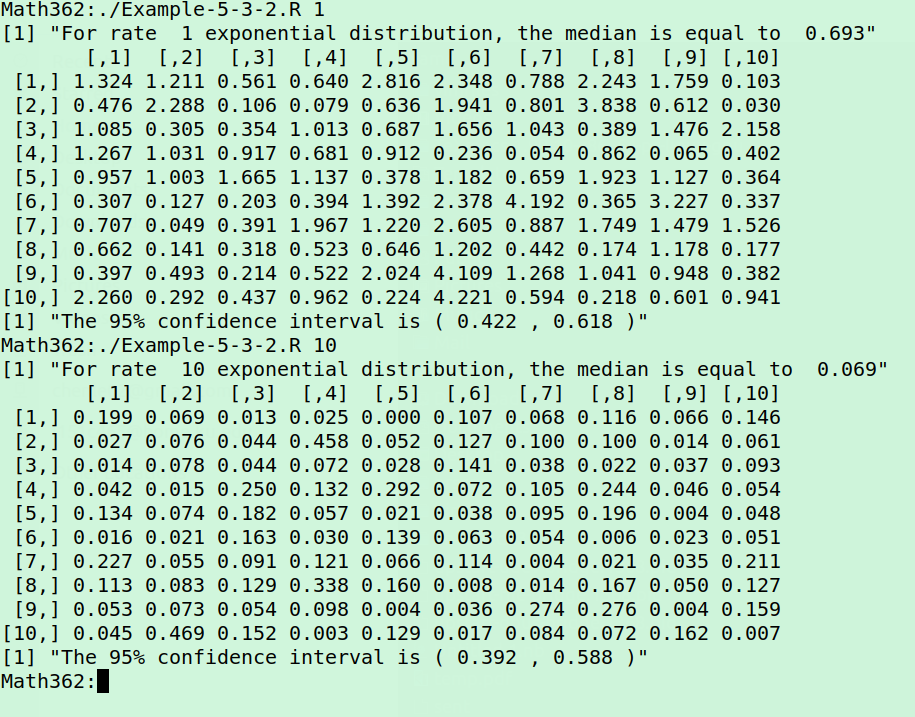
\includegraphics[scale=0.3]{Example-5-3-2-neg.png}
\end{frame}
%-------------- end slide -------------------------------%}}}
%-------------- start slide -------------------------------%{{{ 5.41
\begin{frame}
Instead of the C.I. $\left(\frac{k}{n}-z_{\alpha/2} \sqrt{\frac{(k/n)(1-k/n)}{n}},\:\frac{k}{n}+z_{\alpha/2} \sqrt{\frac{(k/n)(1-k/n)}{n}}\right)$.\\[1em]
One can simply specify the mean $\displaystyle \frac{k}{n}$ and
\[
\text{the {\bf margin of error}:}\qquad  d:=z_{\alpha/2} \sqrt{\frac{(k/n)(1-k/n)}{n}}.
\]
\vfill
\[
\max_{p\in(0,1)} p(1-p)  = p(1-p)\bigg|_{p=1/2} = 1/4 \quad \Longrightarrow \quad d\le \frac{z_{\alpha/2}}{2\sqrt{n}}=:d_m.
\]
\end{frame}
%-------------- end slide -------------------------------%}}}
%-------------- start slide -------------------------------%{{{ 5.42
\begin{frame}
 Comment:
 \begin{enumerate}
  \item When $p$ is close to $1/2$, $d\approx \frac{z_{\alpha/2}}{2\sqrt{n}}$, which is equivalent to $\sigma_p\approx \frac{1}{2\sqrt{n}}$.\\[1em]
 E.g., $n=1000$, $k/n=0.48$, and $\alpha=5\%$, then
 \[
 d=1.96\sqrt{\frac{0.48\times 0.52}{1000}} = 0.0309\underline{7} \quad \text{and}\quad
 d_m = \frac{1.96}{2\sqrt{1000}}= 0.0309\underline{9}
 \]
 \[
 \sigma_p = \sqrt{\frac{0.48\times 0.52}{1000}} =  0.015\underline{7}9873
 \quad \text{and}\quad
 \sigma_p \approx \frac{1}{2\sqrt{1000}}= 0.015\underline{8}1139.
 \]
 \vfill
 \item When $p$ is away from $1/2$, the discrepancy between $d$ and $d_m$ becomes big....
\end{enumerate}
\end{frame}
%-------------- end slide -------------------------------%}}}
%-------------- start slide -------------------------------%{{{ 5.43
\begin{frame}
 \begin{enumerate}
  \item[E.g. ]  Running for presidency. Max and Sirius obtained 480 and 520 votes, respectively. What is probability that Max will win?
  \vfill
  What if the sample size is $n=5000$, and Max obtained 2400 votes.
 \end{enumerate}
\end{frame}
%-------------- end slide -------------------------------%}}}
%-------------- start slide -------------------------------%{{{ 5.44
\begin{frame}{Choosing sample sizes}

 \begin{align}
   d \le  z_{\alpha/2} \sqrt{p(1-p)/n} &\quad\Longleftrightarrow\quad n \ge \frac{z_{\alpha/2}^2p(1-p)}{d^2} \tag{When $p$ is known} \\[1em]
 d \le \frac{z_{\alpha/2}}{2\sqrt{n}} &\quad\Longleftrightarrow\quad n \ge \frac{z_{\alpha/2}^2}{4d^2} \tag{When $p$ is unknown}
 \end{align}
\vfill
\begin{enumerate}
 \item[E.g. ]  Anti-smoking campaign. Need to find an $95\%$ C.I.  with a margin of error equal to $1\%$. Determine the sample size? \\[1em]
 Answer: $n\ge \frac{1.96^2}{4\times 0.01^2} = 9640$.
 \vfill
 \item[E.g.'] In order to reduce the sample size, a small sample is used to determine $p$. One finds that $p\approx 0.22$. Determine the sample size again. \\[1em]
 Answer: $n\ge \frac{1.96^2 \times 0.22\times 0.78}{\times 0.01^2} = 6592.2$.
\end{enumerate}
\end{frame}
%-------------- end slide -------------------------------%}}}

% \section{\S\: 5.4 Properties of Estimators}
% \mySection{5.4 Properties of Estimators}
%-------------- start slide -------------------------------%{{{ 5.48
\begin{frame}{\S\: 5.4 Properties of Estimators}

 {\bf Question:~} Estimators are not in general unique (MLE or MME ...). How to select one estimator?
 \vfill
 {Recall:~} For a random sample of size $n$ from the population with given pdf, we have $X_1,\cdots,X_n$, which are i.i.d. r.v.'s. The estimator $\hat{\theta}$ is a function of $X_i's$:
 \[
 \hat{\theta}=\hat{\theta}(X_1,\cdots,X_n).
 \]
 \vfill
 {\bf Criterions:}
 \begin{enumerate}
   \item Unbiased.\hfill (Mean)
  \item Efficiency, the minimum-variance estimator.\hfill (Variance)
  \item Sufficency.
  \item Consistency. \hfill (Asymptotic behavior)
 \end{enumerate}

 \end{frame}

 \begin{frame}{Unbiasedness}
 \begin{center}
 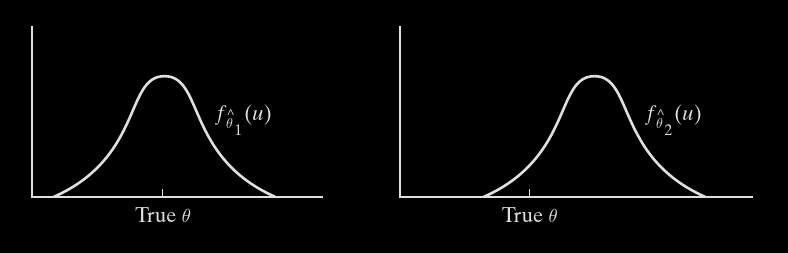
\includegraphics[scale=0.4]{Figure-5-4-2-neg.png}
\end{center}
 \vfill
 {\bf Definition 5.4.1.} Given a random sample of size $n$ whose population distribution dependes on an unknown parameter $\theta$, let $\hat{\theta}$ be an estimator of $\theta$. \\[0.5em]
 Then $\hat{\theta}$ is called {\bf unbiased} if $\E(\hat{\theta}) = \theta$; \\[0.5em]
 and $\hat{\theta}$ is called {\bf asymptotically unbiased} if $\lim_{n\rightarrow\infty}\E(\hat{\theta}) = \theta$.
\end{frame}
%-------------- end slide -------------------------------%}}}
%-------------- start slide -------------------------------%{{{ 5.49
\begin{frame}
\begin{enumerate}
% Ex 5.4.19
\item[E.g. 1.] $f_Y(y;\theta)=\frac{2y}{\theta^2}$ if $y\in [0,\theta]$.
 \begin{itemize}
  \item $\displaystyle\hat{\theta}_1=\frac{3}{2}\overline{Y}$
  \item $\displaystyle\hat{\theta}_2=Y_{max}$.
  \item $\displaystyle\hat{\theta}_3=\frac{2n+1}{2n}Y_{max}$.
 \end{itemize}
 \vfill
 \item[E.g. 2.] Let $X_1,\cdots,X_n$ be a random sample of size $n$ with the unknown parameter $\theta=\E(X)$. Show that for any constants $a_i$'s,
 \[
 \hat{\theta}=\sum_{i=1}^n a_i X_i \quad \text{is unbiased}
 \quad \Longleftrightarrow\quad
 \sum_{i=1}^n a_i=1.
 \]
\end{enumerate}
\end{frame}
%-------------- end slide -------------------------------%}}}
%-------------- start slide -------------------------------%{{{ 5.50
\begin{frame}
 \begin{enumerate}
 \item[E.g. 3.] Let $X_1,\cdots,X_n$ be a random sample of size $n$ with the unknown parameter $\sigma^2=\text{Var}(X)$.
 \begin{itemize}
  \item $\displaystyle \widehat{\sigma}^2=\frac{1}{n}\sum_{i=1}^n \left(X_i-\overline{X}\right)^2$
  \vfill
  \item $\displaystyle S^2= \text{Sample Variance} =\frac{1}{n-1}\sum_{i=1}^n \left(X_i-\overline{X}\right)^2$
  \vfill
  \item $\displaystyle S= \text{Sample Standard Deviation} =\sqrt{\frac{1}{n-1}\sum_{i=1}^n \left(X_i-\overline{X}\right)^2}$. \hfill (Biased for $\sigma$!)
 \end{itemize}
 \vfill
 \end{enumerate}
\end{frame}
%-------------- end slide -------------------------------%}}}
%-------------- start slide -------------------------------%{{{ 5.51
\begin{frame}
\begin{enumerate}
 \item[E.g. 4.] Exponential distr.: $f_Y(y;\lambda)=\lambda e^{-\lambda y}$ for $y\ge 0$. $\widehat{\lambda}=1/\overline{Y}$ is biased.\\[1em] \pause
 $n\overline{Y} = \sum_{i=1}^n Y_i\sim$ Gamma distribution$(n,\lambda)$. \pause Hence,
 \begin{align*}
 \E\left(\widehat{\lambda}\right) &= \E\left(1/\overline{Y}\right) = n\int_0^\infty \frac{1}{y} \frac{\lambda^n}{\Gamma(n)}y^{n-1}e^{-\lambda y}\ud y \\
 \pause& = \frac{n \lambda }{n-1} \int_0^\infty  \underbrace{\frac{\lambda^{n-1}}{\Gamma(n-1)}y^{(n-1)-1}e^{-\lambda y}}_{\text{pdf for Gamma distr. $(n-1,\lambda)$}} \ud y\\
 \pause &= \frac{n}{n-1}\lambda .
 \end{align*}
 Biased! But $\E(\widehat\lambda) = \frac{n}{n-1}\lambda \rightarrow \lambda$ as $n\rightarrow\infty$. (Asymptotically unbiased.)\\[1em]\pause
 Note: ~ $\widehat\lambda^*= \frac{n-1}{n \overline{Y}}$ is unbiased.
 \vfill
 \pause
 \item[E.g. 4'.] Exponential distr.: $f_Y(y;\theta)=\frac{1}{\theta} e^{-y/\theta}$ for $y\ge 0$. $\widehat{\theta}=\overline{Y}$ is unbiased. \\[1em] \pause
\[
\E\left(\widehat{\theta}\right) = \frac{1}{n} \sum_{i=1}^n \E(Y_i) = \frac{1}{n} \sum_{i=1}^n \theta = \theta.
\]
 \end{enumerate}

\end{frame}
%-------------- end slide -------------------------------%}}}
%-------------- start slide -------------------------------%{{{ 5.52
\begin{frame}{Efficiency}
 \begin{center}
 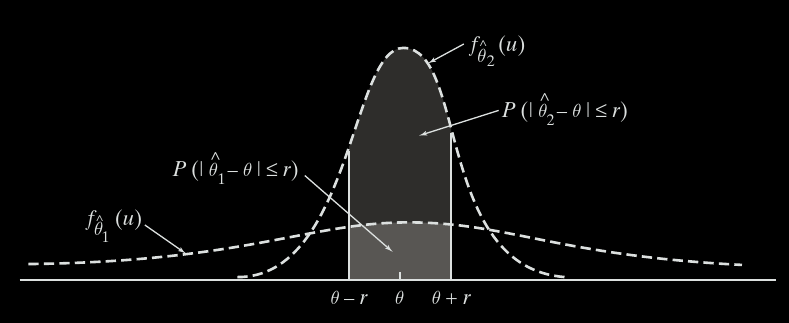
\includegraphics[scale=0.3]{Figure-5-4-3-neg.png}
\end{center}
 \vfill
 {\bf Definition 5.4.2.} Let $\widehat{\theta}_1$ and $\widehat{\theta}_2$ be two unbiased estimators for a parameter $\theta$. If $\Var(\widehat{\theta}_1)<\Var(\widehat{\theta}_2)$, then we say that $\widehat{\theta}_1$ is {\bf more efficient} than $\widehat{\theta}_2$.\\
 The {\bf relative efficiency} of $\widehat{\theta}_1$ w.r.t. $\widehat{\theta}_2$ is the ratio $\Var(\widehat{\theta}_1)/\Var(\widehat{\theta}_2)$.
\end{frame}
%-------------- end slide -------------------------------%}}}
%-------------- start slide -------------------------------%{{{ 5.53
\begin{frame}
 \begin{enumerate}
  \item[E.g. 1.] $f_Y(y;\theta)=\frac{2y}{\theta^2}$ if $y\in [0,\theta]$. Which is more efficient? Find the relative efficiency of $\widehat{\theta}_1$ w.r.t. $\widehat{\theta}_3$ .
 \begin{itemize}
  \item $\displaystyle\hat{\theta}_1=\frac{3}{2}\overline{Y}$ \\[1em]
  \item $\displaystyle\hat{\theta}_3=\frac{2n+1}{2n}Y_{max}$.
 \end{itemize}
 \vfill
 \item[E.g. 2.] Let $X_1,\cdots,X_n$ be a random sample of size $n$ with the unknown parameter $\theta=\E(X)$
	 (suppose $\sigma^2 = \Var(X)<\infty$).\\[1em]
	 \pause
	 Among all possible unbiased estimators $\hat{\theta}=\sum_{i=1}^n a_i X_i$ with $\sum_{i=1}^n a_i=1$.
	 Find the most efficient one.\\[1em]\pause
	 Sol:
 \[
 \Var(\widehat{\theta}) = \sum_{i=1}^n a_i^2 \Var(X) =\sigma^2  \sum_{i=1}^n a_i^2
 \ge \sigma^2 \frac{1}{n} \left(\sum_{i=1}^n a_i\right)^2 = \frac{1}{n} \sigma^2,
 \]
 \[
 \text{with equality iff $a_1=\cdots=a_n=1/n$.}
 \]
 Hence, the most efficient one is the sample mean $\widehat\theta= \overline{X}$.
 \myEnd
 \end{enumerate}

\end{frame}
%-------------- end slide -------------------------------%}}}

% \section{\S\: 5.5 Minimum-Variance Estimators: The Cram\'er-Rao Lower Bound}
% \mySection{5.5 Minimum-Variance Estimators: The Cram\'er-Rao Lower Bound}
%-------------- start slide -------------------------------%{{{ 5.57
\begin{frame}{\S\: 5.5 MVE: The Cram\'er-Rao Lower Bound}

 \hspace{-2em}{\bf Question:~} Can one identify the unbiased estimator having the {\it smallest} variance?
 \vfill
 \hspace{-2em}{\bf Short answer:~} In many cases, yes!
 \vfill
 \begin{center}
 We are going to develop the theory to answer this question in details!
 \end{center}

 \end{frame}

 \begin{frame}

{\bf Regular Estimation/Condition:~} The set of $y$ (resp. $k$) values, where $f_Y(y;\theta)\ne 0$ (resp. $p_X(k;\theta)\ne 0$), does not depend on $\theta$.
\\[1em]
i.e., the domain of the pdf does not depend on the parameter (so that one can differentiate under integration).
 \vfill

 \pause
 {\bf Definition.~} The {\bf Fisher's Information} of a continous (resp. discrete) random variable $Y$ (resp. $X$) with pdf $f_Y(y;\theta)$ (resp. $p_X(k;\theta)$) is defined as
 \[
 I(\theta) = \E\left[\left(\frac{\partial \ln f_Y(Y;\theta)}{\partial \theta}\right)^2\right] \qquad \left(\text{resp.}\quad
 \E\left[\left(\frac{\partial \ln p_X(X;\theta)}{\partial \theta}\right)^2\right]
 \right).
   \]


 \end{frame}
%-------------- end slide -------------------------------%}}}
%-------------- start slide -------------------------------%{{{ 5.58
 \begin{frame}

 {\bf Lemma.~} Under regular condition, let $Y_1,\cdots,Y_n$ be a random sample of size $n$ from the continuous population pdf $f_Y(y;\theta)$. Then the Fisher Information in the random sample $Y_1,\cdots,Y_n$ equals $n$ times the Fisher information in $X$:
 \begin{align}\label{E:Fisher1}
 \E\left[\left(\frac{\partial \ln f_{Y_1,\cdots,Y_n}(Y_1,\cdots,Y_n;\theta)}{\partial \theta}\right)^2\right] = n\:  \E\left[\left(\frac{\partial \ln f_Y(Y;\theta)}{\partial \theta}\right)^2\right] = n \: I(\theta).
 \end{align}
 (A similar statement holds for the  discrete case $p_X(k;\theta)$).\\[1em]

 \pause
 {Proof.~} Based on two observations:
 \[
 LHS = \E\left[\left(
 \sum_{i=1}^n \frac{\partial}{\partial \theta} \ln f_{Y_i}(Y_i;\theta)
 \right)^2\right]
 \]
 \begin{align*}
 \E\left(\frac{\partial}{\partial \theta} \ln f_{Y_i}(Y_i;\theta)\right)
&  = \int_\R \frac{\frac{\partial}{\partial \theta}f_Y(y;\theta)}{f_Y(y;\theta)} f_Y(y;\theta)\ud y = \int_\R \frac{\partial}{\partial \theta}f_Y(y;\theta)\ud y \\
& \stackrel{\text{R.C.}}{=} \frac{\partial}{\partial \theta} \int_\R f_Y(y;\theta)\ud y  = \frac{\partial}{\partial \theta} 1 = 0.
 \end{align*}
\myEnd
 \end{frame}
%-------------- end slide -------------------------------%}}}
%-------------- start slide -------------------------------%{{{ 5.59
 \begin{frame}

  {\bf Lemma.~} Under regular condition, if $\ln f_Y(y;\theta)$ is twice differentiable in $\theta$, then
  \begin{align}\label{E:Fisher2}
  I(\theta) = -\E\left[\frac{\partial^2}{\partial \theta^2}\ln f_Y(Y;\theta)\right].
  \end{align}
(A similar statement holds for the  discrete case $p_X(k;\theta)$).\\[1em]

 \pause
 {Proof.~} This is due to the two facts:
 \[
 \frac{\partial^2}{\partial \theta^2}\ln f_Y(Y;\theta) = \frac{\frac{\partial^2}{\partial \theta^2}f_Y(Y;\theta)}{f_Y(Y;\theta)}
 -\underbrace{\left(\frac{\frac{\partial}{\partial \theta}f_Y(Y;\theta)}{f_Y(Y;\theta)}\right)^2}_{\displaystyle
 =\left(\frac{\partial}{\partial \theta} \ln f_Y(Y;\theta)\right)^2}
 \]
 \begin{align*}
 \E\left(\frac{\frac{\partial^2}{\partial \theta^2}f_Y(Y;\theta)}{f_Y(Y;\theta)}\right) &= \int_\R \frac{\frac{\partial^2}{\partial \theta^2}f_Y(y;\theta)}{f_Y(y;\theta)}f_Y(y;\theta) \ud y =
 \int_\R \frac{\partial^2}{\partial \theta^2}f_Y(y;\theta) \ud y.\\
 &\stackrel{R.C.}{=} \frac{\partial^2}{\partial \theta^2} \int_\R f_Y(y;\theta) \ud y  = \frac{\partial^2}{\partial \theta^2} 1 = 0.
 \end{align*}
 \myEnd
 \end{frame}
%-------------- end slide -------------------------------%}}}
%-------------- start slide -------------------------------%{{{ 5.60
 \begin{frame}

 {\bf Theorem~} (Cram\'er-Rao Inequality)
 Under regular condition, let $Y_1,\cdots,Y_n$ be a random sample of size $n$ from the continuous population pdf $f_Y(y;\theta)$.
Let $\widehat{\theta}=\widehat{\theta}(Y_1,\cdots,Y_n)$ be any unbiased estimator for $\theta$. Then
\[
\Var(\widehat{\theta})\ge \frac{1}{n\:I(\theta)}.
\]

 (A similar statement holds for the  discrete case $p_X(k;\theta)$).\\[1em]

 \pause
 {Proof.~}
If $n=1$, then by Cauchy-Schwartz inequality,
 \begin{align*}
 \E\left[(\widehat{\theta}-\theta) \frac{\partial}{\partial \theta}\ln f_Y(Y;\theta)\right]
 \le \sqrt{\Var(\widehat{\theta})\times I(\theta)}
 \end{align*}
On the other hand,
\begin{align*}
\E\left[(\widehat{\theta}-\theta) \frac{\partial}{\partial \theta}\ln f_Y(Y;\theta)\right] &= \int_\R (\widehat{\theta}-\theta) \frac{\frac{\partial}{\partial \theta} f_Y(y;\theta)}{f_Y(y;\theta)} f_Y(y;\theta)\ud y\\
&= \int_\R (\widehat{\theta}-\theta) \frac{\partial}{\partial \theta} f_Y(y;\theta)\ud y \\
& =\frac{\partial}{\partial \theta} \underbrace{\int_\R (\widehat{\theta}-\theta)  f_Y(y;\theta)\ud y}_{\displaystyle=\E(\widehat{\theta}-\theta)=0}+1=1.
\end{align*}
For general $n$, apply for \eqref{E:Fisher1}. \myEnd.
\end{frame}
%-------------- end slide -------------------------------%}}}
%-------------- start slide -------------------------------%{{{ 5.61
\begin{frame}

{\bf Definition.~} Let $\Theta$ be the set of all estimators $\widehat{\theta}$ that are unbiased for the parameter $\theta$. We say that $\widehat{\theta}^*$ is a {\bf best} or {\bf minimum-variance} esimator (MVE) if $\widehat{\theta}^*\in\Theta$ and
\[
\Var(\widehat{\theta}^*) \le \Var(\widehat{\theta})\qquad \text{for all $\widehat{\theta}\in\Theta$}.
\]
\vfill

{\bf Definition.~} An unbiased estimator $\widehat{\theta}$ is {\bf efficient} if $\Var(\widehat{\theta})$ is equal to the Cram\'er-Rao lower bound, i.e.,  $\Var{\widehat{\theta}} = \left(n\: I(\theta)\right)^{-1}$.\\
The {\bf efficiency} of an unbiased estimator $\widehat{\theta}$ is defined to be $\left(n I(\theta) \Var(\widehat{\theta})\right)^{-1}$.
 \vfill
 \begin{center}
\begin{tikzpicture}[fill=gray,scale=1.4]
\draw[thick,rounded corners] (0,0.15) rectangle (3,2.1);
\fill[gray!20!background] (1.5,1) ellipse (1.4 and 0.75);
\draw (1.5,1) ellipse (1.4 and 0.75);
\fill[red!30!background] (1.2,1) ellipse (0.8 and 0.5);
\draw (1.2,1) ellipse (0.8 and 0.5);
\node at (1.3,1.95) {Unbiased estimators $\Theta$};
\node at (2.4,1) {MVE};
\node at (1.2,1) {Efficient est.};
\end{tikzpicture}
\end{center}
\end{frame}
%-------------- end slide -------------------------------%}}}
%-------------- start slide -------------------------------%{{{ 5.62
\begin{frame}
\begin{enumerate}
 \item[E.g. 1.] $X\sim$Bernoulli(p). Check whether $\widehat{p}=\overline{X}$ is efficient?\\[1em]
 \begin{itemize}
  \item[Step 1.] Compute Fisher's Information:
  \[
 p_X(k;p) = p^k(1-p)^{1-k}.
 \]\pause
 \[
 \ln p_X(k;p) = k\ln p +(1-k)\ln (1-p)
 \]\pause
 \[
 \frac{\partial}{\partial p} \ln p_X(k;p) = \frac{k}{p} -\frac{1-k}{1-p}
 \]\pause
 \[
 -\frac{\partial^2}{\partial^2 p} \ln p_X(k;p) = \frac{k}{p^2} +\frac{1-k}{(1-p)^2}
 \]\pause
 \[
 -\E\left[\frac{\partial^2}{\partial^2 p} \ln p_X(X;p)\right]
 = \E\left[\frac{X}{p^2} +\frac{1-X}{(1-p)^2}\right]
 =\frac{1}{p} + \frac{1}{1-p} =\frac{1}{pq}.
 \]\pause
 \[
 \boxed{I(p) = \frac{1}{pq}, \quad q=1-p.}
 \]
 \item[Step 2.] Compute $\Var(\widehat{p})$.
 \[
 \Var(\widehat{p}) = \frac{1}{n^2}\Var\left(\sum_{i=1}^n X_i\right) = \frac{1}{n^2} n pq = \frac{pq}{n}
 \]
 \item[Conclusion] Because $\widehat{p}$ is unbiased and $ \Var(\widehat{p}) = (n I(p))^{-1}$, $\widehat{p}$ is efficient.
 \end{itemize}
 \end{enumerate}
\end{frame}
%-------------- end slide -------------------------------%}}}
%-------------- start slide -------------------------------%{{{ 5.63
\begin{frame}
\begin{enumerate}
 \item[E.g. 2.] Exponential distr.: $f_Y(y;\lambda)=\lambda e^{-\lambda y}$ for $y\ge 0$. Is $\widehat{\lambda} = 1/\overline{Y}$ efficent?\\[1em]
 \begin{enumerate}
  \item[Answer] No, because  $\widehat{\lambda} $ is biased. Nevertheless, we can still compute Fisher's Information as follows
  \vfill
  \item[Fisher's Inf.]
  \[
 \ln f_Y(y;\lambda) = \ln\lambda -\lambda y
 \]\pause
 \[
 \frac{\partial}{\partial \lambda} \ln f_Y(y;\lambda) = \frac{1}{\lambda} -y
 \]\pause
 \[
 -\frac{\partial^2}{\partial^2 \lambda} \ln f_Y(y;\lambda) = \frac{1}{\lambda^2}
 \]\pause
 \[
 -\E\left[\frac{\partial^2}{\partial^2 \lambda} \ln f_Y(Y;\lambda)\right]
 = \E\left[\frac{1}{\lambda^2} \right]
 =\frac{1}{\lambda^2}.
 \]\pause
 \vfill
 \[\boxed{I(\lambda) = \lambda^{-2}}\]
 \end{enumerate}
 \vfill
 \item[Try:] $\widehat\lambda^*:=\frac{n-1}{n}\frac{1}{\overline{Y}}$. It is unbiased. Is it efficient?
 \end{enumerate}
\end{frame}
%-------------- end slide -------------------------------%}}}
%-------------- start slide -------------------------------%{{{ 5.64
\begin{frame}
\begin{enumerate}
 \item[E.g. 2'.] Exponential distr.: $f_Y(y;\theta)=\theta^{-1} e^{-y/\theta}$ for $y\ge 0$.  $\widehat{\theta}=\overline{Y}$ efficent?\\[1em]
 \begin{itemize}
  \item[Step. 1.] Compute Fisher's Information:
  \[
 \ln f_Y(y;\theta) = -\ln\theta-\frac{y}{\theta}
 \]\pause
 \[
 \frac{\partial}{\partial \theta} \ln f_Y(y;\theta) = -\frac{1}{\theta} +\frac{y}{\theta^2}
 \]\pause
 \[
 -\frac{\partial^2}{\partial^2 \theta} \ln f_Y(y;\theta) = -\frac{1}{\theta^2} + \frac{2y}{\theta^3}
 \]\pause
 \[
 -\E\left[\frac{\partial^2}{\partial^2 \theta} \ln f_Y(Y;\theta)\right]
 = \E\left[-\frac{1}{\theta^2} + \frac{2Y}{\theta^3}  \right]
 =-\frac{1}{\theta^2}+ \frac{2\theta}{\theta^3} = \theta^{-2}.
 \]\pause
  \[\boxed{I(\theta) = \theta^{-2}}\]
 \item[Step 2.] Compute $\Var(\widehat{\theta})$:
 \[
 \Var(\overline{Y}) = \frac{1}{n^2}\sum_{i=1}^n \Var(Y_i) =  \frac{1}{n^2} n \theta^2 = \frac{\theta^2}{n}.
 \]
 \item[Conclusion.] Because $\widehat{\theta}$ is unbiased  and $ \Var(\widehat{p}) = (n I(p))^{-1}$, $\widehat{\theta}$ is efficient.
 \end{itemize}
\end{enumerate}
\end{frame}
%-------------- end slide -------------------------------%}}}
%-------------- start slide -------------------------------%{{{ 5.65
\begin{frame}[label=current]

\begin{enumerate}
 \item[E.g. 3.] $f_Y(y;\theta)=2y/\theta^2$ for $y\in [0,\theta]$.  $\widehat{\theta}=\frac32\overline{Y}$ efficent?\\[1em]
 \begin{itemize}
  \item[Step. 1.] Compute Fisher's Information:
  \[
 \ln f_Y(y;\theta) = \ln (2y)-2\ln\theta
 \]\pause
 \[
 \frac{\partial}{\partial \theta} \ln f_Y(y;\theta) = -\frac{2}{\theta}
 \]\pause
 By the definition of Fisher's information,
 \[
 I(\theta) = \E\left[\left(\frac{\partial}{\partial \theta} \ln f_Y(y;\theta) \right)^2\right]=
 \E\left[\left( - \frac{2}{\theta}  \right)^2\right]= \frac{4}{\theta^2}.
 \] \pause
 However, if we compute
 \[
 -\frac{\partial^2}{\partial^2 \theta} \ln f_Y(y;\theta) = -\frac{2}{\theta^2}
 \]\pause
 \begin{align}\tag{$\dagger$}
 -\E\left[\frac{\partial^2}{\partial^2 \theta} \ln f_Y(Y;\theta)\right]
 = \E\left[-\frac{2}{\theta^2} \right]
 =-\frac{2}{\theta^2} \ne
\frac{4}{\theta^2} = I(\theta) .
 \end{align}
\pause
 \item[Step 2.] Compute $\Var(\widehat{\theta})$:
 \[
 \Var(\widehat\theta) = \frac{9}{4n}\Var(Y) =  \frac{9}{4 n} \frac{\theta^2}{18} = \frac{\theta^2}{8n}.
 \]
 \item[Discussion.] Even though $\widehat\theta$ is unbiased, we have two discripencies: ($\dagger$)  and
 \[
 \Var(\widehat\theta)= \frac{\theta^2}{8n} \le \frac{\theta^2}{4n} = \frac{1}{n I(\theta)}
 \]\pause
 This is because this is not a regular estimation!
 \end{itemize}
\end{enumerate}


\end{frame}
%-------------- end slide -------------------------------%}}}

% \section{\S\: 5.6 Sufficient Estimators}
% \mySection{5.6 Sufficient Estimators}
%-------------- start slide -------------------------------%{{{ 5.69
\begin{frame}{\S\: 5.6 Sufficient Estimators}

 {\bf Rationale:~} Let $\widehat{\theta}$ be an estimator to the unknown parameter $\theta$. Whether does $\widehat{\theta}$ contain all information about $\theta$? \\[1em] \pause
 Equivalently, how can one reduce the random sample of size $n$, denoted by $(X_1,\cdots, X_n)$, to a function without losing any information about $\theta$?

 \vfill
 \pause

 E.g., let's choose the function $h(X_1,\cdots,X_n):= \frac{1}{n}\sum_{i=1}^n X_i$, the sample mean. In many cases, $h(X_1,\cdots,X_n)$ contains all relevant information about the true mean $\E(X)$. In that case, $h(X_1,\cdots,X_n)$, as an estimator, is sufficient.

 \end{frame}

 \begin{frame}

{\bf Definition.~} Let $(X_1,\cdots, X_n)$ be a random sample of size $n$ from a discrete population with a unknown parameter $\theta$, of which $\widehat{\theta}$ (resp. $\theta_e$) be an estimator (resp. estimate).
We call $\widehat\theta$ and $\theta_e$ {\bf sufficient} if
\begin{align}\label{E:Sufficency1}
\tag{Sufficency-1}
\PP\left(X_1=k_1,\cdots, X_n=k_n \: \bigg| \: \widehat\theta = \theta_e\right) = b(k_1,\cdots,k_n)
\end{align}
is a function that does not depend on $\theta$. \\[1em]
In case for random sample $(Y_1,\cdots,Y_n)$ from the continuous population, \eqref{E:Sufficency1} should be
\[
f_{Y_1,\cdots,Y_n |\widehat\theta =\theta_e}\left(y_1,\cdots, y_n \: \bigg| \: \widehat\theta = \theta_e\right) = b(y_1,\cdots,y_n)
\]
\vfill
Note: $\widehat\theta = h(X_1,\cdots, X_n)$ and $\theta_e=h(k_1,\cdots,k_n)$.\\
\qquad or $\widehat\theta = h(Y_1,\cdots, Y_n)$ and $\theta_e=h(y_1,\cdots,y_n)$.
\end{frame}
%-------------- end slide -------------------------------%}}}
%-------------- start slide -------------------------------%{{{ 5.70
\begin{frame}
Equivalently, \\[1em]

{\bf Definition.~}  ... $\widehat\theta$ (or $\theta_e$) is {\bf sufficient} if the likelihood function can be factorized as:
\begin{align}\label{E:Sufficency2}
\tag{Sufficency-2}
L(\theta) =
\begin{cases}
 \displaystyle \prod_{i=1}^n p_X(k_i;\theta) =g(\theta_e,\theta) \: b(k_1,\cdots,k_n) & \text{Discrete}\\[1em]
 \displaystyle \prod_{i=1}^n f_Y(y_i;\theta)=g(\theta_e,\theta) \: b(y_1,\cdots,y_n)& \text{Continous}
\end{cases}
\end{align}
where $g$ is a function of two arguments only and $b$ is a function that does not depend on $\theta$.

\end{frame}
%-------------- end slide -------------------------------%}}}
%-------------- start slide -------------------------------%{{{ 5.71
\begin{frame}
\begin{enumerate}
 \item[E.g. 1.] A random sample of size $n$ from Bernoulli(P). $\widehat p = \sum_{i=1}^n X_i$. Check sufficiency of $\widehat p$ for $p$ by \eqref{E:Sufficency1}:
 \vfill \pause
 Case I: If $k_1,\cdots,k_n\in\{0,1\}$ such that $\sum_{i=1}^n k_i\ne c$, then
 \[
 \PP\left(X_1=k_1,\cdots,X_n=k_n \:\big| \: \widehat p = c \right) = 0.
 \]\pause
 \vfill
 Case II: If $k_1,\cdots,k_n\in\{0,1\}$ such that $\sum_{i=1}^n k_i=c$, then
\end{enumerate}
\end{frame}
%-------------- end slide -------------------------------%}}}
%-------------- start slide -------------------------------%{{{ 5.72
\begin{frame}
 \begin{align*}
  \PP&\left(X_1=k_1,\cdots,X_n=k_n \:\big| \: \widehat p = c \right)\\\pause
  &= \frac{\PP\left(X_1=k_1,\cdots,X_n=k_n, \widehat p = c \right)}{\PP(\widehat p = c)}\\\pause
  &= \frac{\PP\left(X_1=k_1,\cdots,X_n=k_n, X_n + \sum_{i=1}^{n-1} X_i = c \right)}{\PP\left(\sum_{i=1}^n X_i = c\right)}\\ \pause
  &= \frac{\PP\left(X_1=k_1,\cdots,X_{n-1}=k_{n-1}, X_n = c -\sum_{i=1}^{n-1} k_i  \right)}{\PP\left(\sum_{i=1}^n X_i = c\right)}\\ \pause
  &=
  \frac{\left(\prod_{i=1}^{n-1} p^{k_i}(1-p)^{1-k_i}\right) \times p^{c-\sum_{i=1}^{n-1} k_i} (1-p)^{1-c+\sum_{i=1}^{n-1} k_i}}{{n\choose c}p^c(1-p)^{n-c}}\\ \pause
  &=\frac{1}{{n\choose c}}.
 \end{align*}
 \end{frame}
%-------------- end slide -------------------------------%}}}
%-------------- start slide -------------------------------%{{{ 5.73
 \begin{frame}
 In summary,
 \[
 \PP\left(X_1=k_1,\cdots,X_n=k_n \:\big| \: \widehat p = c \right)
 =\begin{cases}
   \frac{1}{{n\choose c}} & \text{if $k_i\in\{0,1\}$ s.t. $\sum_{i=1}^n k_i=c$,}\\
   0 & otherwise.
  \end{cases}
 \]
\vfill \pause
Hence, by \eqref{E:Sufficency1}, $\widehat p = \sum_{i=1}^n X_i$ is a sufficient estimator for $p$.
\end{frame}
%-------------- end slide -------------------------------%}}}
%-------------- start slide -------------------------------%{{{ 5.74
\begin{frame}
\begin{enumerate}
 \item[E.g. 1'.] As in E.g. 1, check sufficiency of $\widehat p$ for $p$ by \eqref{E:Sufficency2}:\\[1em] \pause
Notice that $p_e=\sum_{i=1}^n k_i$. Then \pause
 \begin{align*}
 L( p) = \prod_{i=1}^n p_X(k_i;p) &= \prod_{i=1}^n p^{k_i}(1-p)^{1-k_i}\\ \pause
 &=p^{\sum_{i=1}^n k_i} (1-p)^{n -\sum_{i=1}^n k_i}\\ \pause
 &=p^{p_e} (1-p)^{n -p_e}
%  \\
%  &= \exp\left(p_e \ln p+ (n-p_e) \ln(1-p)\right)
\end{align*}
\pause
Therefore, $p_e$ (or $\widehat p$) is sufficient since \eqref{E:Sufficency2} is satisfied with
\[
g(p_e,p) = p^{p_e} (1-p)^{n -p_e} \quad \text{and}\quad b(k_1,\cdots,k_n) =1.
\] \pause
\vfill
\item[Comment] 1. The estimator $\widehat p$ is sufficient but not unbiased since $\E(\widehat p) = n p \ne p$. \\[0.5em]\pause
2. Any one-to-one function of a sufficient estimator is again a sufficient estimator. E.g., $\widehat p_2:= \frac{1}{n} \widehat p$, which is a unbiased, sufficient, and MVE. \\[0.5em]\pause
3. $\widehat p_3:= X_1$ is not sufficient!
\end{enumerate}
\end{frame}
%-------------- end slide -------------------------------%}}}
%-------------- start slide -------------------------------%{{{ 5.75
\begin{frame}
 \begin{enumerate}
  \item[E.g. 2.] Poisson($\lambda$), $p_X(k;\lambda) =e^{-\lambda}\lambda^k/k!$, $k=0,1,\cdots$. Show that $\widehat\lambda=(\sum_{i=1}^n X_i)^2$ is sufficient for $\lambda$ for a sample of size $n$. \pause
  \vfill
  Sol: The Corresponding estimate is $\lambda_e=(\sum_{i=1}^n k_i)^2$.\pause
  \begin{align*}
   L(\lambda) &= \prod_{i=1}^n \frac{e^{-\lambda}\lambda^{k_i}}{k_i!} \\ \pause
   & = e^{-n\lambda} \lambda^{\sum_{i=1}^n k_i} \left(\prod_{i=1}^n k_i!\right)^{-1}\\ \pause
   & = \underbrace{\mystrut{1.3em} e^{-n\lambda} \lambda^{\sqrt{\lambda_e} }}_{g(\lambda_e,\lambda)} \times \underbrace{\left(\prod_{i=1}^n k_i!\right)^{-1}}_{b(k_1,\cdots,k_n)}.
  \end{align*}\pause
  Hence, $\widehat\lambda$ is sufficient estimator for $\lambda$.\myEnd
  \end{enumerate}
\end{frame}
%-------------- end slide -------------------------------%}}}
%-------------- start slide -------------------------------%{{{ 5.76
\begin{frame}
 \begin{enumerate}
  \item[E.g. 3.] Let $Y_1,\cdots,Y_n$ be a random sample from $f_Y(y;\theta)=\frac{2y}{\theta^2}$ for $y\in [0,\theta]$. Whether is the MLE $\widehat\theta = Y_{max}$ sufficient for $\theta$? \\[1em] \pause
  \vfill
  Sol: The corresponding estimate is $\theta_e= y_{max}$. \pause
  \begin{align*}
   L(\theta) = \prod_{i=1}^n \frac{2y}{\theta^2} I_{[0,\theta]}(y_i) &
   = 2^n\theta^{-2n} \left(\prod_{i=1}^n y_i\right) \times \prod_{i=1}^n I_{[0,\theta]}(y_i)\\ \pause
   &= 2^n\theta^{-2n} \left(\prod_{i=1}^n y_i\right) \times I_{[0,\theta]}(y_{max})\\  \pause
   &= \underbrace{\mystrut{1.5em} 2^n\theta^{-2n}I_{[0,\theta]}(\theta_e)}_{=g(\theta_e,\theta)}  \times \underbrace{\prod_{i=1}^n y_i}_{=b(y_1,\cdots,y_k)}.
  \end{align*} \pause
  Hence, $\widehat\theta$ is a sufficient estimator for $\theta$.\myEnd
  \vfill  \pause
  Note: MME $\widehat\theta = \frac{3}{2}\overline{Y}$ is NOT sufficient for $\theta$!
  \end{enumerate}
\end{frame}
%-------------- end slide -------------------------------%}}}


% \section{\S\: 5.7 Consistency}
% \mySection{5.7 Consistency}
%-------------- start slide -------------------------------%{{{ 5.79
\begin{frame}
  % {\S\: 5.7 Consistency}

 {\bf Definition.~} An estimator $\widehat\theta_n = h(W_1,\cdots,W_n)$ is said
 to be \textcolor{yellow}{consistent} if it converges to $\theta$ {\it in probability}, i.e.,
 for any $\epsilon>0$, \[
		 \lim_{n\rightarrow\infty}\PP\left(|\widehat\theta_n-\theta|<\epsilon\right)=1.
		 \] \vfill \pause Comment: In the $\epsilon$-$\delta$ language, the above
		 \textcolor{yellow}{convergence in probability} says \[ \forall \epsilon>0,\: \forall
				 \delta>0,\:  \exists n(\epsilon,\delta)>0, \: s.t. \: \forall n\ge
				 n(\epsilon,\delta), \] \[
		 \PP\left(|\widehat\theta_n-\theta|<\epsilon\right)>1-\delta.  \]
\end{frame}
%-------------- end slide -------------------------------%}}}
%-------------- start slide -------------------------------%{{{ 5.80
\begin{frame}
 A useful tool to check convergence in probability is
 \vfill

 {\bf Theorem.~} (Chebyshev's inequality) Let $W$ be any r.v. with finite mean $\mu$ and variance $\sigma^2$. Then for any $\epsilon>0$
 \[
 \PP\left(|W-\mu|<\epsilon\right)\ge 1-\frac{\sigma^2}{\epsilon^2},
 \]
 or, equivalently,
 \[
 \PP\left(|W-\mu|\ge \epsilon\right)\le \frac{\sigma^2}{\epsilon^2}.
 \]
 \vfill
 {Proof.} ... \myEnd
\end{frame}
%-------------- end slide -------------------------------%}}}
%-------------- start slide -------------------------------%{{{ 5.81
 \begin{frame}
 As a consequence of Chebyshev's inequality, we have \\
 \vfill
 {\bf Proposition.~} The sample mean $\widehat\mu_n =\frac{1}{n}\sum_{i=1}^n W_i$ is consistent for $\E(W)=\mu$, provided that the population $W$ has finite mean $\mu$ and variance $\sigma^2$.
 \vfill
 Proof.~
 \[
 \E(\widehat \mu_n) = \mu \qquad \text{and} \qquad \Var(\widehat\mu_n)= \frac{\sigma^2}{n}.
 \]
%  For any $\epsilon>0$,
 \[
 \forall \epsilon>0,\quad
 \PP\left(|\widehat\mu_n-\mu|\le \epsilon\right)\ge 1-\frac{\sigma^2}{n\epsilon^2}  \rightarrow 1.
 \]
 \myEnd
 \end{frame}
%-------------- end slide -------------------------------%}}}
%-------------- start slide -------------------------------%{{{ 5.82
\begin{frame}
  \begin{enumerate}
   \item[E.g. 1.~] Let $Y_1,\cdots, Y_n$ be a random sample of size $n$ from the uniform pdf $f_Y(y;\theta) = 1/\theta$, $y\in [0,\theta]$. Let $\widehat\theta_n =Y_{max}$. We know that $Y_{max}$ is biased. Is it consistent?
   \vfill \pause
   {\noindent\bf Sol.~} The c.d.f. of $Y$ is equal to $F_Y(y) = y/\theta$ for $y\in[0,\theta]$. \pause Hence,
   \[
   f_{Y_{max}}(y) = n F_{Y}(y)^{n-1} f_Y(y) = \frac{n y^{n-1}}{\theta^n}, \qquad y\in [0,\theta].
   \] \pause
   Therefore,
   \begin{align*}
    \bbP(|\widehat\theta_n -\theta|<\epsilon) & = \bbP(\theta-\epsilon< \widehat\theta_n < \theta+\epsilon)\\ \pause
					      &= \int_{\theta-\epsilon}^\theta \frac{n y^{n-1}}{\theta^n }\ud y + \int_{\theta}^{\theta+\epsilon} 0 \ud y\\ \pause
    &= 1- \left(\frac{\theta-\epsilon}{\theta}\right)^n \\ \pause
    & \rightarrow 0 \quad \text{as $n\rightarrow\infty$.}
   \end{align*}
   \myEnd
  \end{enumerate}
 \end{frame}
%-------------- end slide -------------------------------%}}}
%-------------- start slide -------------------------------%{{{ 5.83
\begin{frame}
 \begin{enumerate}
  \item[E.g. 2.~]  Suppose $Y_1 , Y_2 , \cdots, Y_n$ is a random sample from the
exponential pdf, $f_Y (y; \lambda) = \lambda e^{-\lambda y}$, $y > 0$.
Show that $\widehat\lambda_n = Y_1$ is not consistent for $\lambda$.
\vfill
 {\noindent\bf Sol.~}
 To prove $\widehat\lambda_n$ is not consistent for $\lambda$, we need only to find out one $\epsilon>0$ such that the following limit does not hold:
\begin{align}\label{E:573}
\lim_{n\rightarrow\infty} \bbP\left(|\widehat\lambda_n -\lambda|<\epsilon\right)=1.
\end{align} \pause
We can choose $\epsilon = \lambda/m$ for any $m\ge 1$. Then
\begin{align*}
|\widehat\lambda_n - \lambda| \le \frac{\lambda}{m}
& \quad\Longleftrightarrow\quad
\left(1-\frac{1}{m}\right)\lambda \le \widehat\lambda_n \le \left(1+\frac{1}{m}\right)\lambda
\\ \pause
& \quad \Longrightarrow \quad
\widehat\lambda_n \ge \left(1-\frac{1}{m}\right)\lambda.
\end{align*}
 \end{enumerate}
\end{frame}
%-------------- end slide -------------------------------%}}}
%-------------- start slide -------------------------------%{{{ 5.84
\begin{frame}
\begin{enumerate}
 \item[] Hence,
\begin{align*}
\bbP\left(|\widehat\lambda_n -\lambda|<\frac{\lambda}{m}\right)
& \le \bbP\left(\widehat\lambda_n \ge \left(1-\frac{1}{m}\right)\lambda \right)\\ \pause
& = \bbP\left(Y_1\ge \left(1-\frac{1}{m}\right)\lambda \right)\\ \pause
&= \int_{\left(1-\frac{1}{m}\right)\lambda }^\infty \lambda e^{-\lambda y}\ud y\\ \pause
&= e^{-\left(1-\frac{1}{m}\right)\lambda^2}<1.
\end{align*}
Therefore, the limit in \eqref{E:573} cannot hold. \myEnd
\end{enumerate}
\end{frame}
%-------------- end slide -------------------------------%}}}

% \section{\S\: 5.8 Bayesian Estimation}
% \mySection{5.8 Bayesian Estimation}
%-------------- start slide -------------------------------%{{{ 5.87
\begin{frame}
  % {\S\: 5.8 Bayesian Estimation}

{\bf Rationale:~} Let $W$ be an estimator dependent on a parameter $\theta$.
\begin{enumerate}
 \item Frequentists view $\theta$ as a parameter whose exact value is to be estimated.\\[1em]
 \item Bayesians view $\theta$ is the value of a random variable $\Theta$. \\[1em]
 \pause
 One can incorporate our knowledge on $\Theta$ --- the {\bf prior distribution} $p_\Theta(\theta)$ if $\Theta$ is discrete and $f_\Theta(\theta)$ if $\Theta$ is continuous --- and use Bayes' formula to update our knowledge on $\Theta$ upon new observation $W=w$:
%  \vfill
\begin{align*}
g_\Theta(\theta|W=w)=
\begin{cases}
 \displaystyle \frac{p_W(w|\Theta=\theta) p_\Theta(\theta)}{\PP(W=w)} & \text{if $W$ is discrete} \\[2em]
 \displaystyle \frac{f_W(w|\Theta=\theta) f_\Theta(\theta)}{f_W(w)}   & \text{if $W$ is continuous}
\end{cases}
 \end{align*}
 where $g_\Theta(\theta|W=w)$ is called {\bf posterior distribution} of $\Theta$.
\end{enumerate}
\end{frame}
%-------------- end slide -------------------------------%}}}
%-------------- start slide -------------------------------%{{{ 1
\begin{frame}[fragile]
\begin{center}
  \tikzset{every node/.append style={scale=0.9}}
  \tikzset{
      invisible/.style={opacity=0},
      visible on/.style={alt={#1{}{invisible} }},
      alt/.code args={<#1>#2#3}{%
        \alt<#1>{\pgfkeysalso{#2}}{\pgfkeysalso{#3}} % \pgfkeysalso doesn't change the path
      },
    }
  \tikzset{level 1 concept/.append style={font=\sf, sibling angle=90,level distance = 15em}}
  % \tikzset{level 2 concept/.append style={font=\sf, sibling angle=45,level distance = 15mm}}
  \begin{tikzpicture}[mindmap,concept color=black,text=black]

\def\colorTotal{red!80!black}
\def\colorPrior{green!80!black}
\def\colorL{yellow!80!black}
\def\colorPost{blue!80!black}
  \begin{scope}[concept color=red!30!black]
    \node[text width=14em,scale=1,text=white] (right) at (2.2,0) {$\Huge\displaystyle \textcolor{\colorPost}{P(\Theta|W)} = \frac{\textcolor{\colorL}{P(W\mid \Theta)}\textcolor{\colorPrior}{P(\Theta)}}{\textcolor{\colorTotal}{P(W)}}$}
    [counterclockwise from=45]
    child[concept color=\colorPrior] { node[concept] {Prior distribution of $\Theta$}}
    child[concept color=\colorL] { node[concept] {Likelihood of sample $W$} }
    child[concept color=\colorPost] { node[concept] {Posterior of $\Theta$} }
    child[concept color=\colorTotal] { node[concept] {Total Probability of sample $W$} }
  ;
  \end{scope}
  \end{tikzpicture}
\end{center}
\end{frame}
%-------------- end slide -------------------------------%}}}
%-------------- start slide -------------------------------%{{{ 5.88
 \begin{frame}{Four cases for computing posterior distribution}
 \begin{center}
 \def\arraystretch{4}
  \begin{tabular}{ l | c | c }
    \hline
  $g_\Theta(\theta|W=w)$ \cellcolor{gray!50!background} & $W$ discrete  \cellcolor{gray!50!background}                                                                             & $W$ continuous  \cellcolor{gray!50!background}                                                                          \\ \hline
  $\Theta$ discrete  \cellcolor{gray!50!background}     & $\displaystyle \frac{p_W(w|\Theta=\theta) p_\Theta(\theta)}{\sum_{i} p_W(w|\Theta=\theta_i) p_\Theta(\theta_i)}$         & $\displaystyle \frac{f_W(w|\Theta=\theta) p_\Theta(\theta)}{\sum_{i} f_W(w|\Theta=\theta_i) p_\Theta(\theta_i)}$        \\ \hline
  $\Theta$ continuous \cellcolor{gray!50!background}    & $\displaystyle \frac{p_W(w|\Theta=\theta) f_\Theta(\theta)}{\int_\R p_W(w|\Theta=\theta') f_\Theta(\theta')\ud \theta'}$ & $\displaystyle \frac{f_W(w|\Theta=\theta) f_\Theta(\theta)}{\int_\R f_W(w|\Theta=\theta') f_\Theta(\theta')\ud\theta'}$ \\ \hline
  \end{tabular}
\end{center}
\end{frame}
%-------------- end slide -------------------------------%}}}
%-------------- start slide -------------------------------%{{{ 5.89
\begin{frame}{Gamma distributions}
\[
\Gamma(r) := \int_0^\infty y^{r-1} e^{-y} \ud y,\quad r>0.
\] \pause
\vfill
Two parametrizations for {\bf Gamma distributions}:
\vfill
\begin{enumerate}
  \item With a \textcolor{magenta}{shape parameter} $r$ and a \textcolor{blue}{scale parameter} $\theta$:
 \[
 f_Y(y;r,\theta) =  \frac{y^{r-1} e^{-y/\theta}}{\theta^r \Gamma(r)},
 \qquad y>0, r,\theta>0.
 \]
 \vfill
 \item With a \textcolor{magenta}{shape parameter} $r$ and a \textcolor{yellow}{rate parameter} $\lambda=1/\theta$,
 \[
 f_Y(y;r,\lambda) = \frac{\lambda^r y^{r-1} e^{-\lambda y}}{\Gamma(r)},
 \qquad y>0, r,\lambda>0.
 \]
 \vfill
 \item[]
 \[
 \E[Y] =  \frac{r}{\lambda} = r\theta \quad \text{and}\quad
 \Var(Y) = \frac{r}{\lambda^2} = r\theta^2
 \]
\end{enumerate}

\end{frame}
%-------------- end slide -------------------------------%}}}
%-------------- start slide -------------------------------%{{{ 5.90
\begin{frame}[fragile]

 \begin{center}
  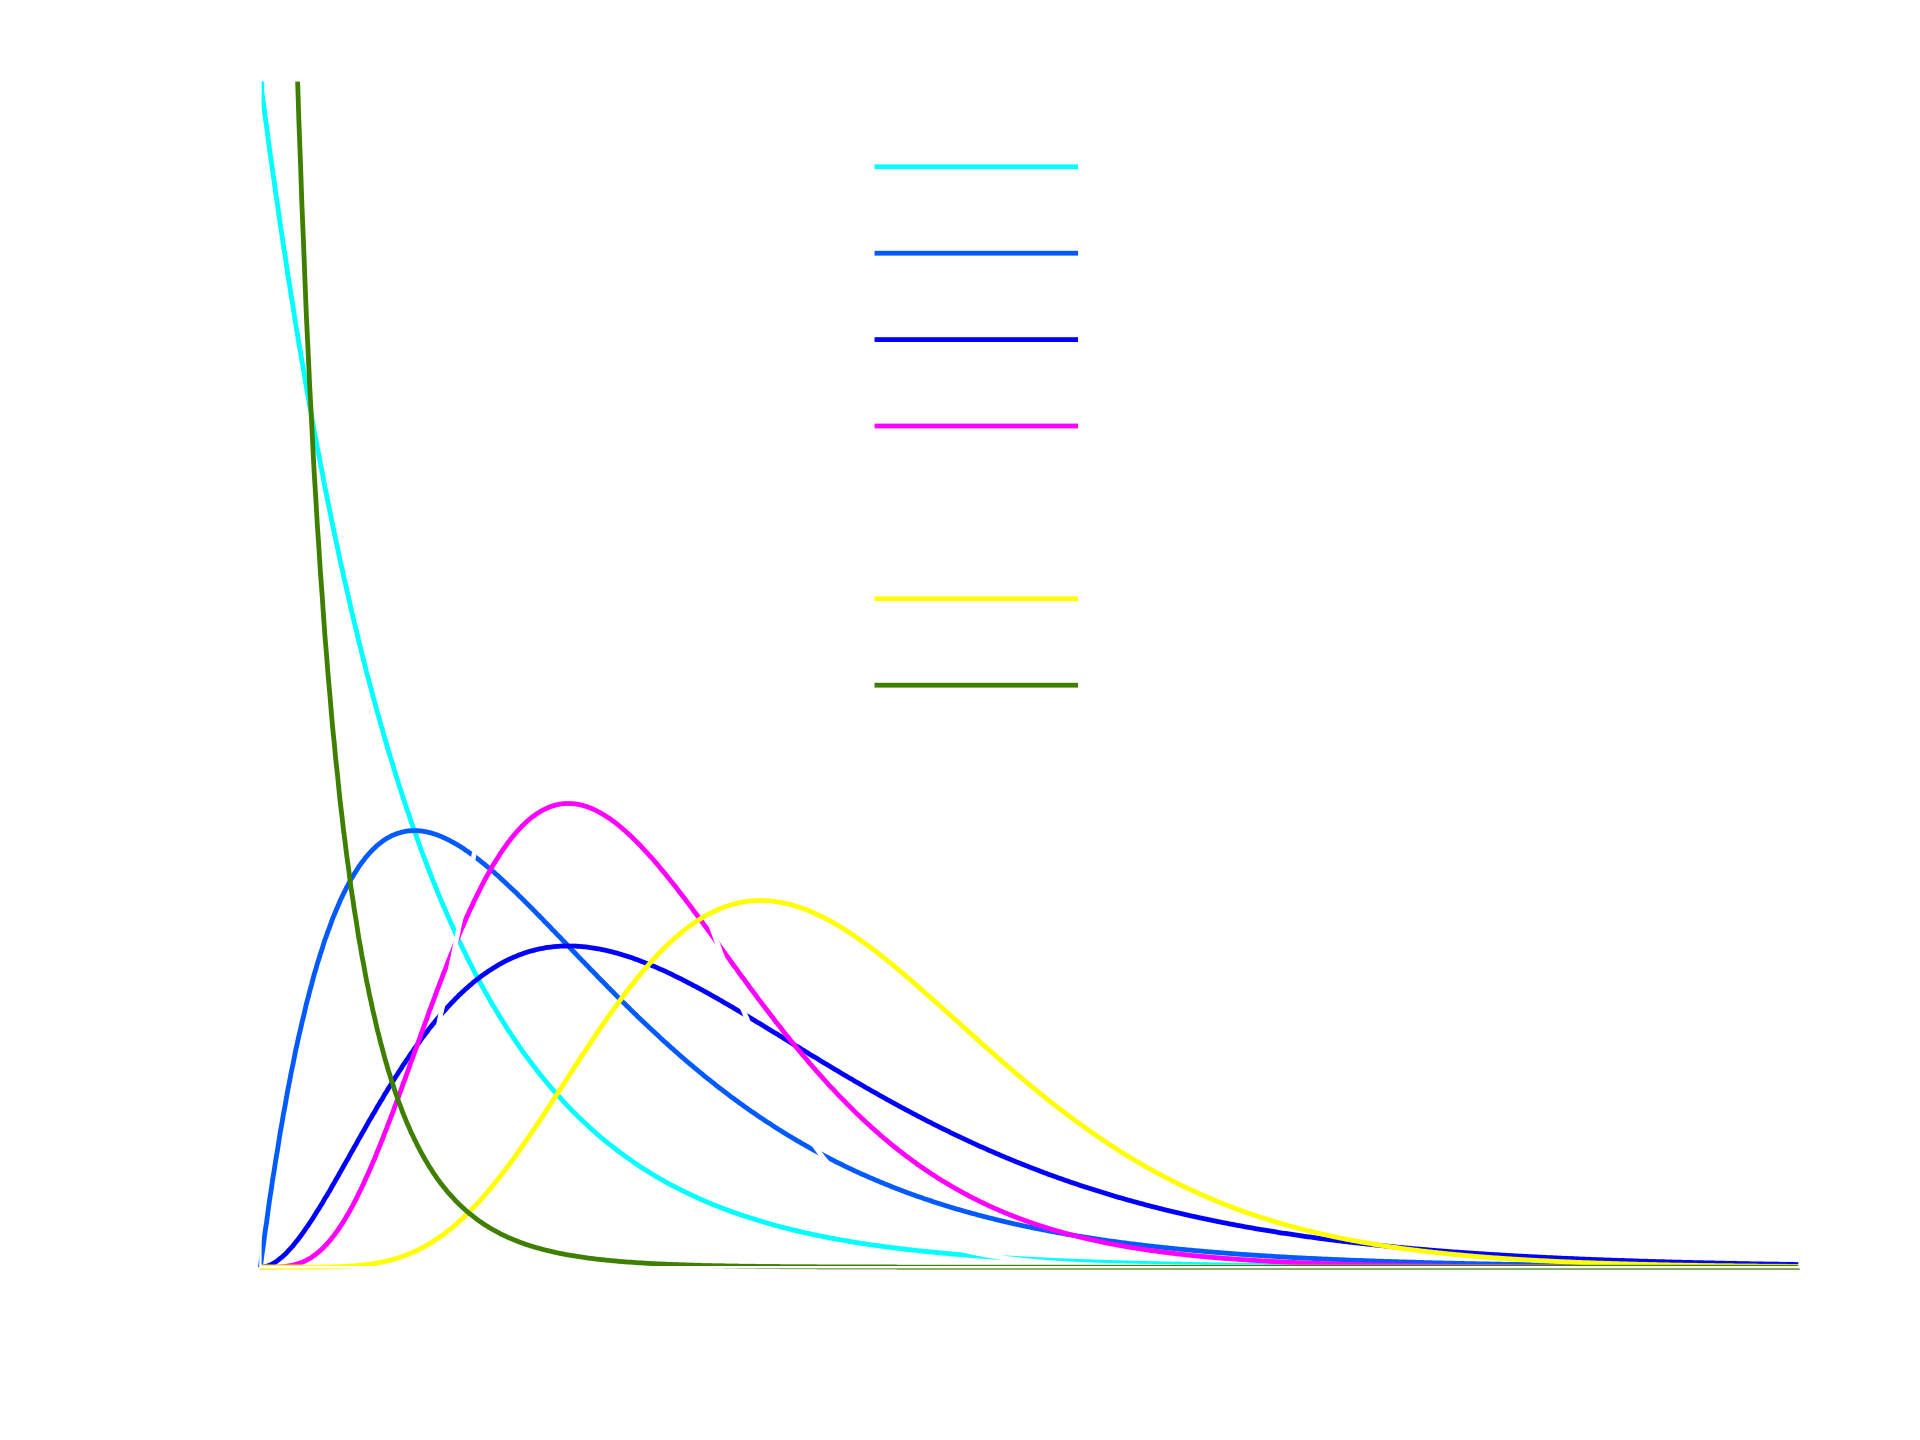
\includegraphics[scale=0.11]{1920px-Gamma_distribution_pdf.svg-neg.png}
  \begin{minipage}{0.4\textwidth}
  \begin{lstlisting}
# Plot gamma distributions
x = seq(0,20,0.01)
k= 3 # Shape parameter
theta = 0.5 # Scale parameter
plot(x,dgamma(x, k, scale = theta),
     type="l",
     col="red")
  \end{lstlisting}
  \end{minipage}
 \end{center}

\end{frame}
%-------------- end slide -------------------------------%}}}
%-------------- start slide -------------------------------%{{{ 5.91
\begin{frame}{Beta distributions}
 \begin{align*}
 B(\alpha,\beta) := & \int_0^1 y^{\alpha-1}(1-y)^{\beta-1}\ud y, \quad \alpha,\beta >0. \\ \pause
 \vdots& \qquad \vdots \\ \pause
 =& \frac{\Gamma(\alpha)\Gamma(\beta)}{\Gamma(\alpha+\beta)}. \qquad\qquad  \text{\textcolor{gray}{\small (see Appendix)}}
 \end{align*}
\vfill \pause
Beta distribution
\[
f_Y(y;\alpha,\beta) = \frac{y^{\alpha-1}(1-y)^{\beta-1}}{B(\alpha,\beta)}, \quad y\in[0,1], \alpha,\beta>0.
\]
\vfill \pause
\[
\E[Y] = \frac{\alpha}{\alpha+\beta}\quad\text{and}\quad
\Var(Y) = \frac{\alpha\beta}{(\alpha+\beta)^2(\alpha+\beta+1)}
\]
\end{frame}
%-------------- end slide -------------------------------%}}}
%-------------- start slide -------------------------------%{{{ 5.92
\begin{frame}[fragile]

\begin{center}
 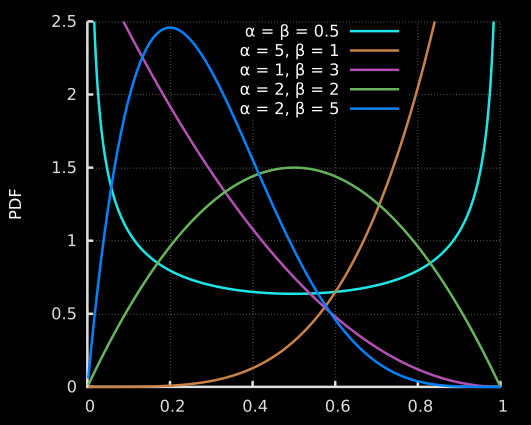
\includegraphics[scale=0.375]{Beta_distribution_pdf-neg.png}\\
 \vfill
 \begin{minipage}{0.4\textwidth}
  \begin{lstlisting}
   # Plot Beta distributions
x = seq(0,1,0.01)
a = 13
b = 2
plot(x,dbeta(x,a,b),
     type="l",
     col="red")
  \end{lstlisting}
 \end{minipage}
\end{center}

\end{frame}
%-------------- end slide -------------------------------%}}}
%-------------- start slide -------------------------------%{{{ 5.93
\begin{frame}
\begin{enumerate}
 \item[E.g. 1.]  Let $X_1,\cdots, X_n$ be a random sample from Bernoulli$(\theta)$: $p_{X_i}(k;\theta) = \theta^k(1-\theta)^{1-k}$ for $k=0,1$.\\[1em]  \pause
 Let $X=\sum_{i=1}^n X_i$. \pause
 Then $X$ follows binomial$(n, \theta)$. \\[1em] \pause
 Prior distribution: $\Theta\sim$beta$(r,s)$, i.e., $f_\Theta(\theta)=\frac{\Gamma(r+s)}{\Gamma(r)\Gamma(s)}\theta^{r-1}(1-\theta)^{s-1}$ for $\theta\in [0,1]$. \\ \pause
 \vfill
\begin{minipage}{0.45\textwidth}
\begin{eqnarray*}
 X_1,\cdots, X_n \:\big| \theta &\sim &\text{Bernoulli$(\theta)$}\\
 \Theta & \sim& \text{Beta$(r,s)$}\\
 && \text{$r$ \& $s$ are known}
\end{eqnarray*}
\end{minipage}
\hfill
\begin{minipage}{0.45\textwidth}
\begin{eqnarray*}
 X=\sum_{i=1}^nX_i \: \bigg| \theta&\sim& \text{Binomial$(n,\theta)$}\\
 \Theta & \sim& \text{Beta$(r,s)$}\\
 && \text{$r$ \& $s$ are known}
\end{eqnarray*}
\end{minipage}
\end{enumerate}
\end{frame}
%-------------- end slide -------------------------------%}}}
%-------------- start slide -------------------------------%{{{ 5.94
\begin{frame}
 \begin{center}
 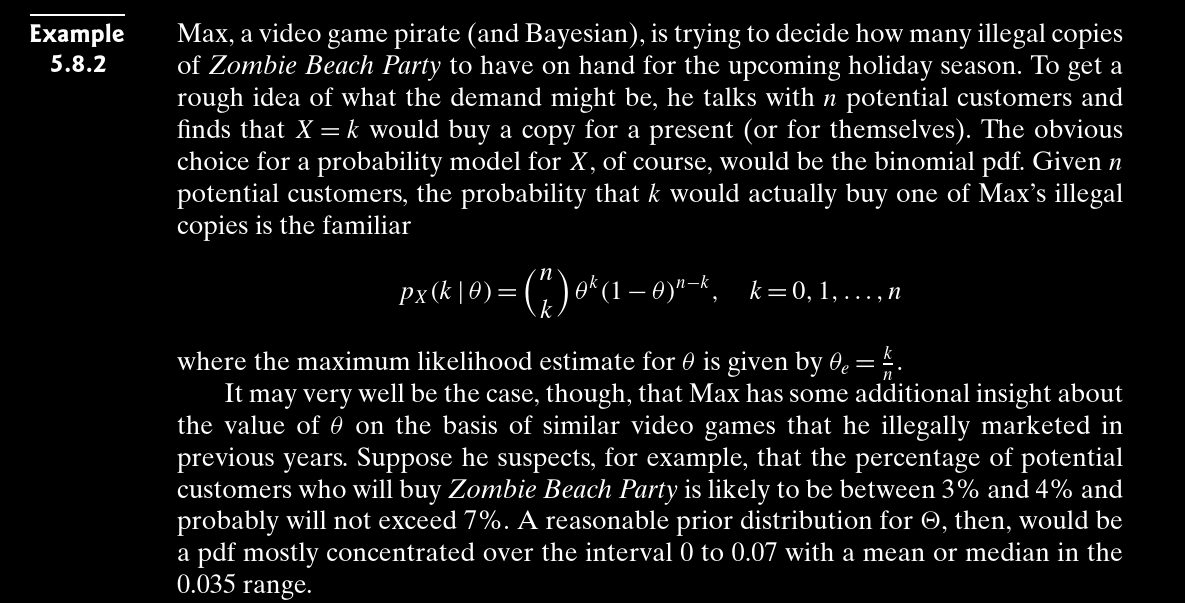
\includegraphics[scale=0.26]{Example-5-8-2-neg.png}
\end{center}
\end{frame}
%-------------- end slide -------------------------------%}}}
%-------------- start slide -------------------------------%{{{ 5.95
\begin{frame}
\begin{center}
 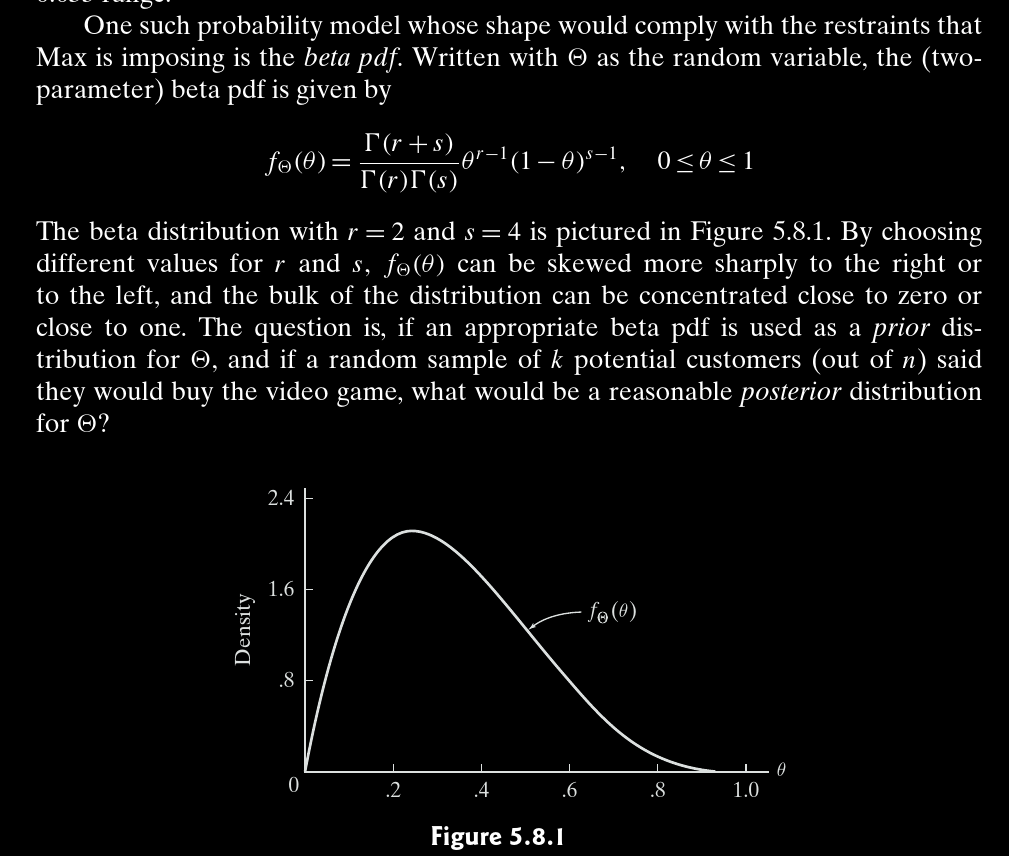
\includegraphics[scale=0.26]{Example-5-8-2-2-neg.png}
\end{center}

\end{frame}
%-------------- end slide -------------------------------%}}}
%-------------- start slide -------------------------------%{{{ 5.96
\begin{frame}
  $X$ is discrete and $\Theta$ is continuous.
  \[
 g_\Theta(\theta|X=k) = \frac{p_X(k|\Theta=\theta) f_\Theta(\theta)}{\int_\R p_X(k|\Theta=\theta') f_\Theta(\theta')\ud \theta'}
  \] \pause
  \begin{align*}
  p_X(k|\Theta=\theta) f_\Theta(\theta)
  &= {n\choose k} \theta^k (1-\theta)^{n-k} \times \frac{\Gamma(r+s)}{\Gamma(r)\Gamma(s)}\theta^{r-1}(1-\theta)^{s-1}\\ \pause
  &= {n\choose k} \frac{\Gamma(r+s)}{\Gamma(r)\Gamma(s)} \theta^{k+r-1} (1-\theta)^{n-k+s-1},\quad \theta\in[0,1].
  \end{align*}\pause
\begin{align*}
p_X(k) =& \int_\R p_X(k|\Theta=\theta') f_\Theta(\theta') \ud\theta'\\ \pause
=& {n\choose k} \frac{\Gamma(r+s)}{\Gamma(r)\Gamma(s)}  \int_0^1 \theta'^{k+r-1} (1-\theta')^{n-k+s-1}\ud \theta'\\ \pause
=& {n\choose k} \frac{\Gamma(r+s)}{\Gamma(r)\Gamma(s)}  \times \frac{\Gamma(k+r)\Gamma(n-k+s)}{\Gamma((k+r)+(n-k+s))}
\end{align*}
\end{frame}
%-------------- end slide -------------------------------%}}}
%-------------- start slide -------------------------------%{{{ 5.97
\begin{frame}
 \begin{align*}
  g_\Theta(\theta|X=k) =& \frac{\displaystyle {n\choose k} \frac{\Gamma(r+s)}{\Gamma(r)\Gamma(s)} \times \theta^{k+r-1} (1-\theta)^{n-k+s-1}}{\displaystyle {n\choose k} \frac{\Gamma(r+s)}{\Gamma(r)\Gamma(s)}  \times \frac{\Gamma(k+r)\Gamma(n-k+s)}{\Gamma((k+r)+(n-k+s))}} \\ \pause
  = & \frac{\Gamma(n+r+s)}{\Gamma(k+r)\Gamma(n-k+s)} \theta^{k+r-1} (1-\theta)^{n-k+s-1}, \qquad \theta\in[0,1]
 \end{align*} \pause
 \vfill
Conclusion: the posterior $\sim$ beta distribution$(k+r, n-k+s)$. \\[1em]
Recall that the prior $\sim$ beta distribution$(r, s)$.
\end{frame}
%-------------- end slide -------------------------------%}}}
%-------------- start slide -------------------------------%{{{ 5.98
\begin{frame}

It remains to determine the values of $r$ and $s$ to incorporate the prior knowledge: \\[1em]
\begin{enumerate}
 \item[PK 1.] Mean is about 0.035.
 \[
\E(\Theta) = 0.035 \quad\Longrightarrow\quad \frac{r}{r+s} = 0.035 \quad \Longleftrightarrow \quad \frac{r} {s}= \frac{7}{193}
\]
\vfill
\item[PK 2.] The pdf mostly concentrated over $[0,0.07]$. ... trial ...
\end{enumerate}
\end{frame}
%-------------- end slide -------------------------------%}}}
%-------------- start slide -------------------------------%{{{ 5.99
\begin{frame}[fragile]

\begin{minipage}{0.45\textwidth}
  \begin{lstlisting}
x <- seq(0, 1, length = 1025)
plot(x,dbeta(x,4,102),
     type="l")
plot(x,dbeta(x,7,193),
     type="l")
dev.off()

pdf=cbind(dbeta(x,4,102),dbeta(x,7,193))
matplot(x,pdf,
        type="l",
        lty = 1:2,
        xlab = "theta", ylab = "PDF",
        lwd = 2 # Line width
        )
legend(0.2, 25, # Position of legend
       c("Beta(4,102)", "Beta(7,193)"),
       col = 1:2, lty = 1:2,
       ncol = 1, # Number of columns
       cex = 1.5, # Fontsize
       lwd=2 # Line width
       )
abline(v=0.07, col="blue", lty=1,lwd=1.5)
text(0.07, -0.5, "0.07")
abline(v=0.035, col="gray60", lty=3,lwd=2)
text(0.035, 1, "0.035")
\end{lstlisting}
\end{minipage}
\begin{minipage}{0.5\textwidth}
  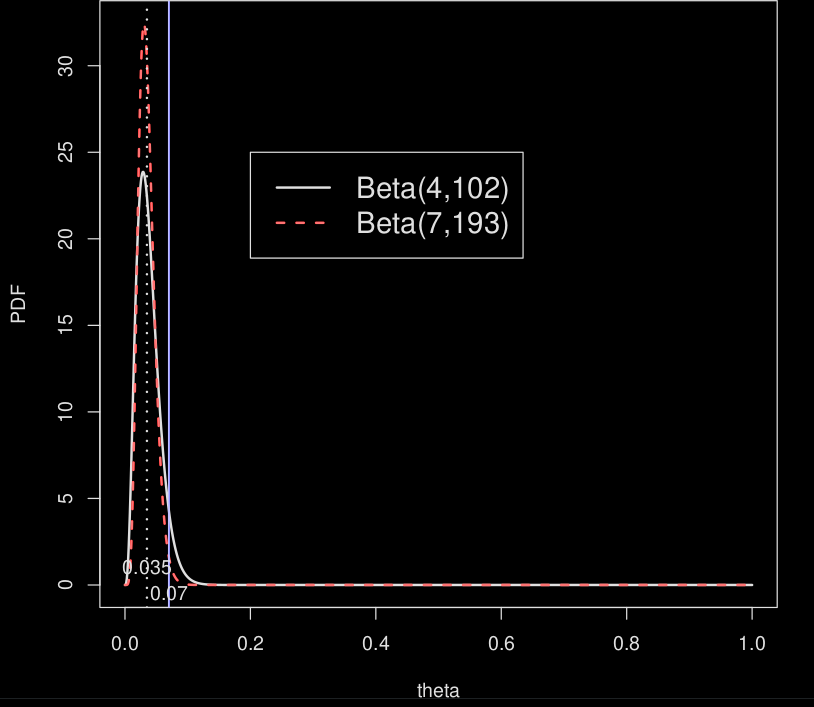
\includegraphics[scale=0.24]{BetaPrior_neg.png}
\end{minipage}
\end{frame}
%-------------- end slide -------------------------------%}}}
%-------------- start slide -------------------------------%{{{ 5.100
\begin{frame}
If we choose $r=7$ and $s=193$:
 \begin{align*}
  g_\Theta(\theta|X=k) = & \frac{\Gamma(n+200)}{\Gamma(k+7)\Gamma(n-k+193)} \theta^{k+6} (1-\theta)^{n-k+192}, \qquad \theta\in[0,1]
 \end{align*}
 \vfill
 Moreover, if $n=10$ and $k=2$,
  \begin{align*}
  g_\Theta(\theta|X=k) = & \frac{\Gamma(210)}{\Gamma(9)\Gamma(201)} \theta^{8} (1-\theta)^{200}, \qquad \theta\in[0,1]
 \end{align*}
\end{frame}
%-------------- end slide -------------------------------%}}}
%-------------- start slide -------------------------------%{{{ 5.101
\begin{frame}[fragile]

\begin{minipage}{0.45\textwidth}
 \begin{lstlisting}
x <- seq(0, 0.1, length = 1025)
pdf=cbind(dbeta(x,7,193),dbeta(x,9,201))
matplot(x,pdf,
        type="l",
        lty = 1:2,
        xlab = "theta", ylab = "PDF",
        lwd = 2 # Line width
)
legend(0.05, 25, # Position of legend
       c("Posterior Beta(9,201)", "Prior Beta(7,193)"),
       col = 1:2, lty = 1:2,
       ncol = 1, # Number of columns
       cex = 1.5, # Fontsize
       lwd=2 # Line width
)
abline(v=0.07,col="blue", lty=1,lwd=1.5)
text(0.07, -0.5, "0.07")
abline(v=0.035,col="black", lty=3,lwd=2)
text(0.035, 1, "0.035")
 \end{lstlisting}
\end{minipage}
\begin{minipage}{0.5\textwidth}
 \centering
 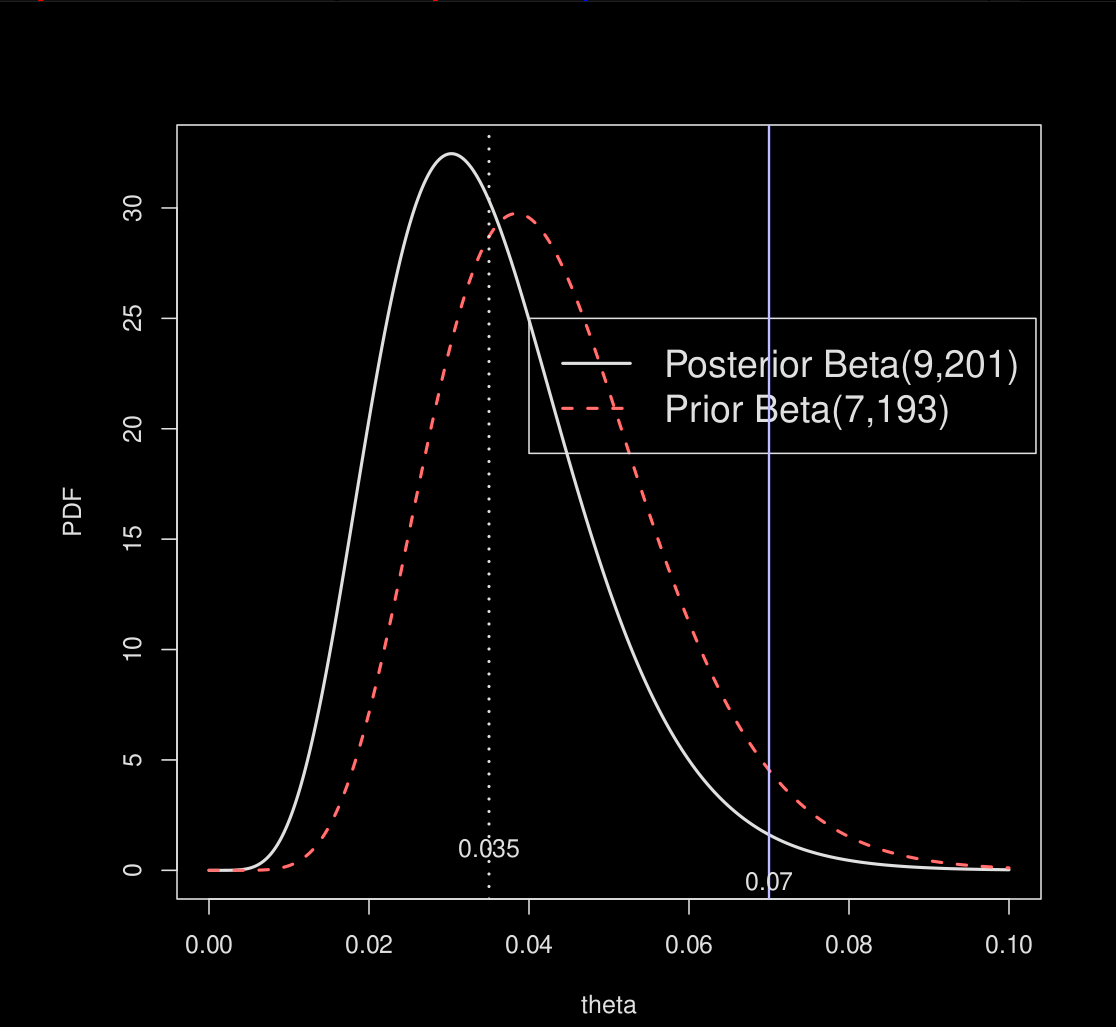
\includegraphics[scale=0.16]{BetaPriorPosterior_neg.png}
\end{minipage}
 \end{frame}

 \begin{frame}

 {\bf Definition.~} If the posterior distributions $p(\Theta| X)$ are in the same probability distribution family as the prior probability distribution $p(\Theta)$,
 the prior and posterior are then called \textcolor{magenta}{conjugate distributions}, and the prior is called a \textcolor{magenta}{conjugate prior} for the likelihood function.

 \vfill
 \begin{enumerate}
  \item Beta distributions are conjugate priors for Bernoulli, \underline{binomial}, nega. binomial, geometric  likelihood.
  \\[1em]
  \item Gamma distributions are conjugate priors for \underline{Poisson} and exponential likelihood.
 \end{enumerate}

\end{frame}
%-------------- end slide -------------------------------%}}}
%-------------- start slide -------------------------------%{{{ 5.102
\begin{frame}

\begin{enumerate}
 \item[E.g. 2.] Let $X_1,\cdots, X_n$ be a random sample from Poisson$(\theta)$: $p_X(k;\theta) = \frac{e^{-\theta}\theta^k}{k!}$ for $k=0,1,\cdots$.\\[1em]  \pause
 Let $W=\sum_{i=1}^n X_i$. \pause
 Then $W$ follows Poisson$(n\theta)$. \\[1em] \pause
 Prior distribution: $\Theta\sim$ Gamma$(s,\mu)$, i.e., $f_\Theta(\theta)=\frac{\mu^s}{\Gamma(s)}\theta^{s-1}e^{-\mu\theta}$ for $\theta>0$. \\[1em]\pause
%  Posterior Gamma$(w+s,\mu+n)$ upon observing $W=w$.
\end{enumerate}
\vfill
\begin{minipage}{0.45\textwidth}
\begin{eqnarray*}
 X_1,\cdots, X_n \:\big| \theta &\sim &\text{Poisson$(\theta)$}\\
 \Theta & \sim& \text{Gamma$(s,\mu)$}\\
 && \text{$s$ \& $\mu$ are known}
\end{eqnarray*}
\end{minipage}
\hfill
\begin{minipage}{0.45\textwidth}
\begin{eqnarray*}
 W=\sum_{i=1}^nX_i \: \bigg| \theta&\sim& \text{Poisson$(n\theta)$}\\
 \Theta & \sim& \text{Gamma$(s,\mu)$}\\
 && \text{$s$ \& $\mu$ are known}
\end{eqnarray*}
\end{minipage}
\end{frame}
%-------------- end slide -------------------------------%}}}
%-------------- start slide -------------------------------%{{{ 5.103
\begin{frame}
  \[
 g_\Theta(\theta|W=w) = \frac{p_W(w|\Theta=\theta) f_\Theta(\theta)}{\int_\R p_W(w|\Theta=\theta') f_\Theta(\theta')\ud \theta'}
  \]
  \vfill \pause
  \begin{align*}
  p_W(w|\Theta=\theta) f_\Theta(\theta)
  &= \frac{e^{-n\theta}(n\theta)^w}{w!}\times \frac{\mu^s}{\Gamma(s)}\theta^{s-1}e^{-\mu\theta}\\ \pause
  &= \frac{n^w}{w!} \frac{\mu^s}{\Gamma(s)}\times \theta^{w+s-1}e^{-(\mu+n)\theta}, \quad \theta>0.
  \end{align*}
\vfill \pause
  \begin{align*}
p_W(w) =& \int_\R p_W(w|\Theta=\theta') f_\Theta(\theta') \ud\theta'\\ \pause
=& \frac{n^w}{w!} \frac{\mu^s}{\Gamma(s)} \int_0^\infty \theta'^{w+s-1}e^{-(\mu+n)\theta'}\ud \theta'\\\pause
=& \frac{n^w}{w!} \frac{\mu^s}{\Gamma(s)} \times \frac{\Gamma(w+s)}{(\mu+n)^{w+s}}
\end{align*}
\end{frame}
%-------------- end slide -------------------------------%}}}
%-------------- start slide -------------------------------%{{{ 5.104
\begin{frame}
 \begin{align*}
  g_\Theta(\theta|X=k) =& \frac{\displaystyle \frac{n^w}{w!} \frac{\mu^s}{\Gamma(s)} \times \theta^{w+s-1}e^{-(\mu+n)\theta}}{\displaystyle  \frac{n^w}{w!} \frac{\mu^s}{\Gamma(s)} \times \frac{\Gamma(w+s)}{(\mu+n)^{w+s} }} \\
  = & \frac{(\mu+n)^{w+s}}{\Gamma(w+s)} \theta^{w+s-1}e^{-(\mu+n)\theta}, \qquad \theta>0.
 \end{align*}
 \vfill
Conclusion: the posterior of $\Theta$ $\sim$ gamma distribution$(w+s, n+\mu)$. \\[1em]
Recall that the prior of $\Theta$ $\sim$ gamma distribution$(s, \mu)$.
\end{frame}
%-------------- end slide -------------------------------%}}}
%-------------- start slide -------------------------------%{{{ 5.105
\begin{frame}[fragile]{Case Study 5.8.1}

 \begin{minipage}{0.45\textwidth}
 \begin{lstlisting}
x <- seq(0, 4, length = 1025)
pdf=cbind(dgamma(x, shape=88, rate=50),
          dgamma(x, shape=88+92, 100),
          dgamma(x, 88+92+72, 150))
matplot(x,pdf,
        type="l",
        lty = 1:3,
        xlab = "theta", ylab = "PDF",
        lwd = 2 # Line width
)
legend(2, 3.5, # Position of legend
       c("Prior Gamma(88,50)",
         "Posterior1 Beta(180,100)",
         "Posterior2 Beta(252,150)"),
       col = 1:3, lty = 1:3,
       ncol = 1, # Number of columns
       cex = 1.5, # Fontsize
       lwd=2 # Line width
)
 \end{lstlisting}
 \end{minipage}
\begin{minipage}{0.5\textwidth}
 \begin{center}
 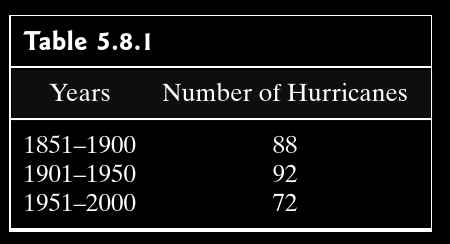
\includegraphics[scale=0.2]{Table-5-8-1-neg.png}
 \vspace{-2em}
 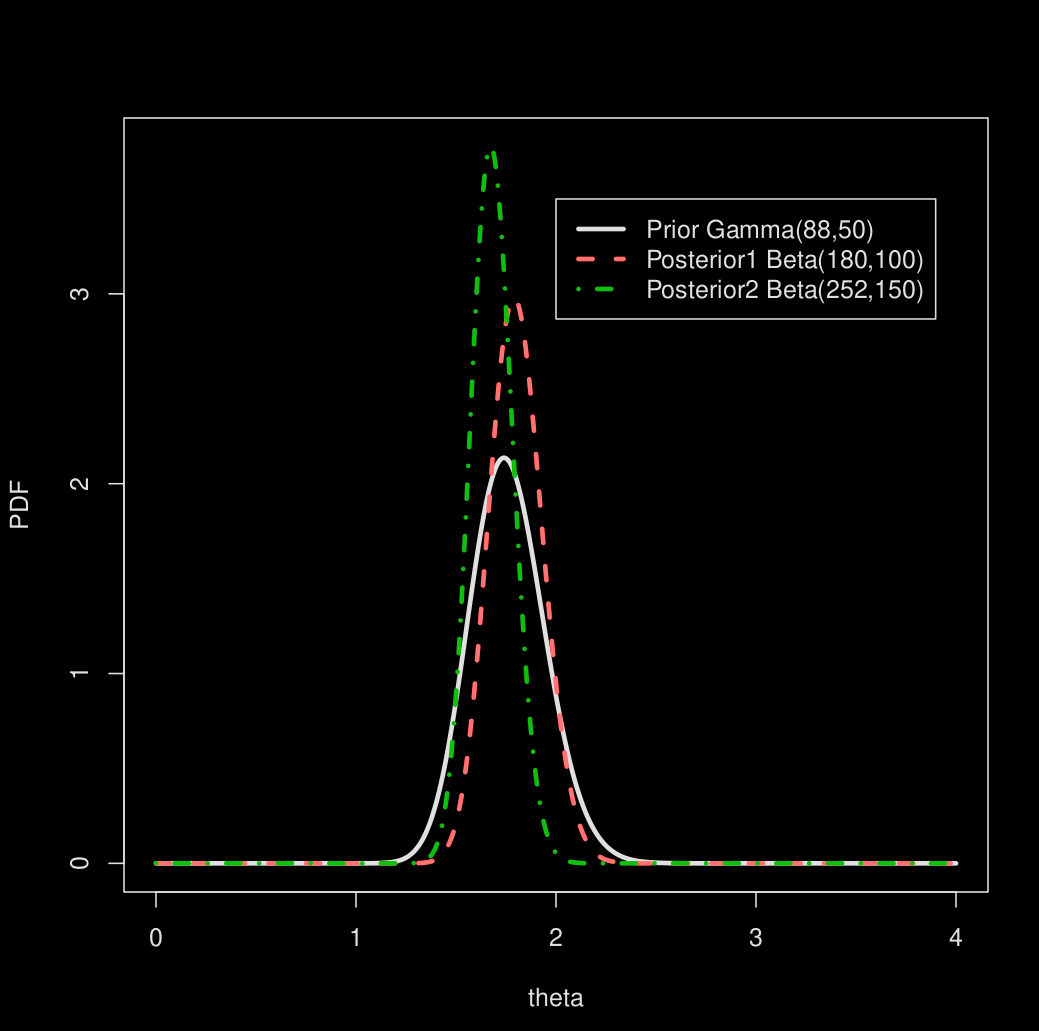
\includegraphics[scale=0.15]{GammaPriorPosterior_neg.png}
 \end{center}
\end{minipage}
\end{frame}
%-------------- end slide -------------------------------%}}}
%-------------- start slide -------------------------------%{{{ 5.106
\begin{frame}{Bayesian Point Estimation}

 {\bf Question.~} Can one calculate an appropriate {\em point estimate} $\theta_e$ given the posterior $g_\Theta(\theta|W=w)$?
 \vfill \pause
 {\bf Definitions.~}
Let $\theta_e$ be an estimate for $\theta$ based on a statistic $W$.
The \textcolor{magenta}{loss function} associated with $\theta_e$ is denoted $L(\theta_e,\theta)$, where $L(\theta_e,\theta)\ge 0$
and $L(\theta, \theta)=0$. \\[1em]\pause
Let $g_\Theta(\theta|W=w)$ be the posterior distribution of the random variable $\Theta$.
Then the \textcolor{magenta}{risk} associated with $\widehat\theta$ is
\textcolor{yellow}{the expected value of the loss function} with respect to the posterior distribution of $\Theta$:
\[
\text{risk}=
\begin{cases}
 \displaystyle \int_\R L(\widehat\theta,\theta) g_\Theta(\theta|W=w)\ud \theta & \text{if $\Theta$ is continuous}\\[1em]
 \displaystyle \sum_{i} L(\widehat\theta,\theta_i) g_\Theta(\theta_i|W=w)& \text{if $\Theta$ is discrete}
\end{cases}
\]
\end{frame}
%-------------- end slide -------------------------------%}}}
%-------------- start slide -------------------------------%{{{ 5.107
\begin{frame}

 {\bf Theorem.} Let $g_\Theta(\theta|W=w)$ be the posterior distribution of the random variable $\Theta$. \\[1em]
 \begin{enumerate}
  \item If $L(\theta_e,\theta)=|\theta_e-\theta|$, then the Bayes point estimate for $\theta$ is the \textcolor{magenta}{median} of  $g_\Theta(\theta|W=w)$.\\[1em]
  \item If $L(\theta_e,\theta)=(\theta_e-\theta)^2$, then the Bayes point estimate for $\theta$ is the \textcolor{yellow}{mean} of  $g_\Theta(\theta|W=w)$.
 \end{enumerate}
 \vfill \pause
%  {\noindent Proof.} ...... \myEnd
 \vfill
\pause
Remarks
\begin{enumerate}
 \item \textcolor{magenta}{Median} usually does not have a closed form formula.
 \item \textcolor{yellow}{Mean} usually has a closed formula.
\end{enumerate}
\end{frame}
%-------------- end slide -------------------------------%}}}
%-------------- start slide -------------------------------%{{{ 5.108
\begin{frame}
\centering

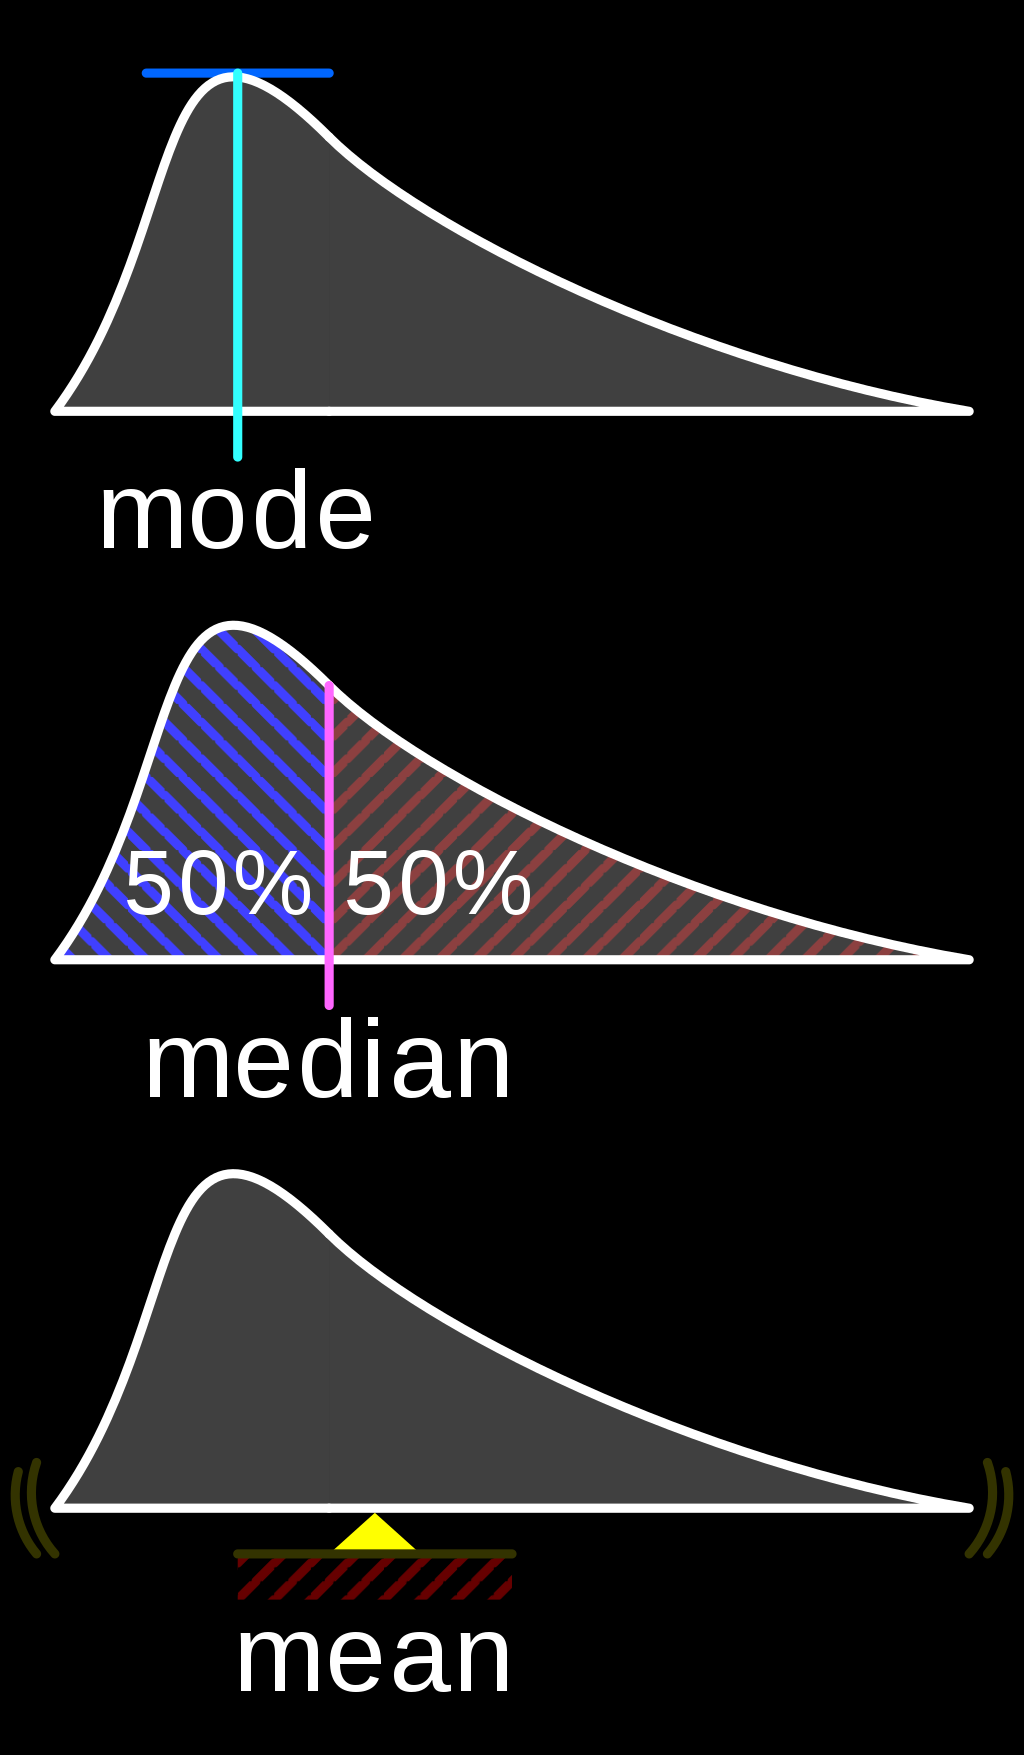
\includegraphics[scale=0.09]{Visualisation_mode_median_mean.svg-neg.png}

\vfill
\footnotesize
\url{https://en.wikipedia.org}
\end{frame}
%-------------- end slide -------------------------------%}}}
%-------------- start slide -------------------------------%{{{ 5. Proof part 1.
\begin{frame}[fragile]

\begin{proofnoend}[ of Part 1. ]
Let $m$ be the \textcolor{magenta}{median} of the random variable $W$. We first claim that
\begin{align}
  \label{E:Median}\tag{$\star$}
  \E(|W-m|)\le \E(|W|).
\end{align}
For any constant $b\in\R$, because
\begin{align*}
  \frac{1}{2} =\bbP(W\le m) = \bbP(W-b\le m-b)
\end{align*}
we see that $m-b$ is the \textcolor{magenta}{median} of $W-b$. Hence, by \eqref{E:Median},
\begin{align*}
  \E\left(|W-m|\right) =\E\left(|(W-b)-(m-b)|\right) \le \E\left(|W-b|\right),\quad \text{for all $b\in\R$},
\end{align*}
which proves the statement.
\end{proofnoend}
\end{frame}
%-------------- end slide -------------------------------%}}}
%-------------- start slide -------------------------------%{{{ 5. Proof of part 1.
\begin{frame}[fragile]
\begin{proofnoend}[ of Part 1. continued ]
It remains to prove \eqref{E:Median}. Without loss of generality, we may assume $m>0$. Then
\begin{align*}
  \E(|W-m|) & = \int_\R |w-m|f_W(w)dw \\
            & = \int_{-\infty}^m (m-w)f_W(w)dw + \int_m^\infty(w-m)f_W(w)dw\\
            & = - \int_{-\infty}^m wf_W(w)dw + \int_m^\infty w\: f_W(w)dw + \frac{1}{2}(m-m)\\
            & = - \int_{-\infty}^0 wf_W(w)dw - \underbrace{\int_{0}^m wf_W(w)dw}_{\ge 0}  + \int_m^\infty w\: f_W(w)dw \\
            & \le - \int_{-\infty}^0 wf_W(w)dw   + \int_{\alert{0}}^\infty w\: f_W(w)dw \\
            & = \int_{\R} |w| f_W(w)dw \\
            & = \E(|W|).
  \end{align*}
  \myQED
 \end{proofnoend}
\end{frame}
%-------------- end slide -------------------------------%}}}
%-------------- start slide -------------------------------%{{{ 5. Proof of part 2.
\begin{frame}[fragile]
  \begin{proofnoend}[ of Part 2. ]
    Let $\mu$ be the \textcolor{yellow}{mean} of  $W$. Then for any $b\in\R$, we see that
     \begin{align*}
      \E\left[(W-b)^2\right] & = \E\left[\left([W-\mu]+[\mu-b]\right)^2\right] \\
                             & = \E\left[(W-\mu )^2\right] + 2 (\mu-b)\underbrace{\E(W-\mu)}_{=0} +[\mu-b]^2 \\
                             & = \E\left[(W-\mu )^2\right] +[\mu-b]^2 \\[1em]
                             & \ge  \E\left[(W-\mu )^2\right],
    \end{align*}
    that is,
\begin{align*}
       \E\left[(W-\mu)^2\right] \le  \E\left[(W-b)^2\right], \quad \text{for all $b\in\R$.}
\end{align*}
    \myQED
  \end{proofnoend}
\end{frame}
%-------------- end slide -------------------------------%}}}
%-------------- start slide -------------------------------%{{{ 5.109
\begin{frame}

\begin{enumerate}
\item[E.g. 1'.]
\begin{minipage}{0.45\textwidth}
\begin{eqnarray*}
 X_1,\cdots, X_n \:\big| \theta &\sim &\text{Bernoulli$(\theta)$}\\
 \Theta & \sim& \text{Beta$(r,s)$}\\
 && \text{$r$ \& $s$ are known}
\end{eqnarray*}
\end{minipage}
\hfill
\begin{minipage}{0.45\textwidth}
\begin{eqnarray*}
 X=\sum_{i=1}^nX_i \: \bigg| \theta&\sim& \text{Binomial$(n,\theta)$}\\
 \Theta & \sim& \text{Beta$(r,s)$}\\
 && \text{$r$ \& $s$ are known}
\end{eqnarray*}
\end{minipage} \pause\pause
\vfill
Prior Beta$(r,s)$ $\rightarrow$ posterior Beta$(k+r, n-k+s)$\\ \pause
upon observing $X=k$ for a random sample of size $n$.  \\[1em] \pause
Consider the $L^2$ loss function.
 \begin{align*}
 \theta_e & =\text{mean of Beta$(k+r,n-k+s)$} \\ \pause
 &= \frac{k+r}{n+r+s}\\ \pause
 &= \frac{n}{n+r+s}\times \underbrace{\mystrut{1em}\left(\frac{k}{n}\right)}_{\text{MLE}} + \frac{r+s}{n+r+s} \times \underbrace{\left(\frac{r}{r+s}\right)}_{\text{Mean of Prior}}
 \end{align*}
 \end{enumerate}
 \end{frame}
%-------------- end slide -------------------------------%}}}
%-------------- start slide -------------------------------%{{{ MLE vs. Prior
\begin{frame}[fragile]
\begin{center}
  MLE vs. Prior

 
\includegraphics[scale=0.25]{./Codes/tug_war.png}
\end{center}
\[\theta_e\]
\[||\]
\begin{align*}
 \frac{n}{n+r+s}\times \underbrace{\mystrut{1em}\left(\frac{k}{n}\right)}_{\text{MLE}} + \frac{r+s}{n+r+s} \times \underbrace{\left(\frac{r}{r+s}\right)}_{\text{Mean of Prior}}
 \end{align*}
\end{frame}
%-------------- end slide -------------------------------%}}}
%-------------- start slide -------------------------------%{{{ 5.110
\begin{frame}
\begin{enumerate}
 \item[E.g. 2'.]
\begin{minipage}{0.45\textwidth}
\begin{eqnarray*}
 X_1,\cdots, X_n \:\big| \theta &\sim &\text{Poisson$(\theta)$}\\
 \Theta & \sim& \text{Gamma$(s,\mu)$}\\
 && \text{$s$ \& $\mu$ are known}
\end{eqnarray*}
\end{minipage}
\hfill
\begin{minipage}{0.45\textwidth}
\begin{eqnarray*}
 W=\sum_{i=1}^nX_i \: \bigg| \theta&\sim& \text{Poisson$(n\theta)$}\\
 \Theta & \sim& \text{Gamma$(s,\mu)$}\\
 && \text{$s$ \& $\mu$ are known}
\end{eqnarray*}
\end{minipage} \pause
\vfill
Prior Gamma$(s,\mu)$ $\rightarrow$ Posterior Gamma$(w+s,\mu+n)$ \\ \pause
 upon observing $W=w$ for a random sample of size $n$.  \\[1em] \pause
Consider the $L^2$ loss function.
 \begin{align*}
 \theta_e & =\text{mean of Gamma$(w+s,\mu+n)$} \\ \pause
 &= \frac{w+s}{\mu +n}\\ \pause
 &= \frac{n}{\mu+n}\times \underbrace{\mystrut{1em}\left(\frac{w}{n}\right)}_{\text{MLE}} + \frac{\mu}{\mu+n} \times \underbrace{\left(\frac{s}{\mu}\right)}_{\text{Mean of Prior}}
 \end{align*}
 \end{enumerate}
\end{frame}
%-------------- end slide -------------------------------%}}}
%-------------- start slide -------------------------------%{{{ MLE vs. Prior
\begin{frame}[fragile]
\begin{center}
  MLE vs. Prior

 
\includegraphics[scale=0.25]{./Codes/tug_war.png}
\end{center}
\[\theta_e\]
\[||\]
\begin{align*}
 \frac{n}{\mu+n}\times \underbrace{\mystrut{1em}\left(\frac{w}{n}\right)}_{\text{MLE}} + \frac{\mu}{\mu+n} \times \underbrace{\left(\frac{s}{\mu}\right)}_{\text{Mean of Prior}}
 \end{align*}
\end{frame}
%-------------- end slide -------------------------------%}}}
%-------------- start slide -------------------------------%{{{ 5.111
\begin{frame}{Appendix: Beta integral}

	 {\bf Lemma.~} $\quad \displaystyle B(\alpha,\beta): = \int_0^1 x^{\alpha-1}(1-x)^{\beta-1}\ud x = \frac{\Gamma(\alpha)\Gamma(\beta)}{\Gamma(\alpha+\beta)}$
	 \vfill
	 {\bf Proof.}
 Notice that
 \[
 \Gamma(\alpha) = \int_0^\infty x^{\alpha-1}e^{-x}dx
 \quad\text{and}\quad
 \Gamma(\beta) = \int_0^\infty y^{\beta-1}e^{-y}dy.
 \]
 Hence,
 \[
 \Gamma(\alpha)\Gamma(\beta)
 = \int_0^\infty\int_0^\infty x^{\alpha-1}y^{\beta-1}e^{-(x+y)}dxdy.
 \]
 \end{frame}

 \begin{frame}
 The key in the proof is the following change of variables:
\vfill
 \[
 \begin{cases}
 x = r^2 \cos^2(\theta)\\
 y = r^2 \sin^2(\theta)
 \end{cases}
 \]
\vfill
 \[
 \Longrightarrow \quad
	 \frac{\partial (x,y)}{\partial (r,\theta)}
 =\begin{pmatrix}
   2r \cos^2(\theta) & 2r\sin^2(\theta) \\
   -2r^2 \cos(\theta)\sin(\theta) & 2r^2 \cos(\theta)\sin(\theta)
  \end{pmatrix}
 \]
\vfill
 \[
 \Longrightarrow \quad \left|\det\left(
 \frac{\partial (x,y)}{\partial (r,\theta)}\right)
 \right| = 4r^3 \sin(\theta)\cos(\theta).
 \]
 \end{frame}
%-------------- end slide -------------------------------%}}}
%-------------- start slide -------------------------------%{{{ 5.112
\begin{frame}
 Therefore,
  \begin{align*}
 \Gamma(\alpha)\Gamma(\beta)
 = &
 \int_0^{\frac{\pi}{2}}d\theta \int_0^\infty dr \:
 r^{2(\alpha+\beta)-4} e^{-r^2} \cos^{2\alpha-2}(\theta)\sin^{2\beta-2}(\theta) \times \underbrace{4 r^3 \sin(\theta) \cos(\theta)}_{\text{Jacobian}}\\
 = & 4 \left(\int_0^{\frac{\pi}{2}}
 \cos^{2\alpha-1}(\theta)\sin^{2\beta-1}(\theta)d\theta \right)
 \left(\int_0^\infty r^{2(\alpha+\beta)-1}e^{-r^2}dr\right).
 \end{align*}
 \vfill
 Now let us compute the following two integrals separately:
\vfill

\begin{align*}
	I_1 &:=\int_0^{\frac{\pi}{2}}
 \cos^{2\alpha-1}(\theta)\sin^{2\beta-1}(\theta)d\theta
 \\[1em]
	I_2 &:= \int_0^\infty r^{2(\alpha+\beta)-1}e^{-r^2}dr
\end{align*}

\end{frame}
%-------------- end slide -------------------------------%}}}
%-------------- start slide -------------------------------%{{{ 5.113
\begin{frame}
For $I_2$, by change of variable $r^2 = u$ (so that $2rdr =du$),
\vfill
\begin{align*}
	I_2 &  =
\int_0^\infty r^{2(\alpha+\beta)-1}e^{-r^2}dr\\
&= \frac{1}{2}\int_0^\infty r^{2(\alpha+\beta)-2}e^{-r^2} \underbrace{2rdr}_{=du}\\
&= \frac{1}{2}\int_0^\infty u^{\alpha+\beta-1}e^{-u}du\\
&=\frac{1}{2} \Gamma(\alpha+\beta).
\end{align*}
\end{frame}
%-------------- end slide -------------------------------%}}}
%-------------- start slide -------------------------------%{{{ 5.114
\begin{frame}
For $I_1$, by the change of variables $\sqrt{x}=\cos(\theta)$ (so that $-\sin(\theta)d\theta = \frac{1}{2\sqrt{x}}dx$),
\vfill
\begin{align*}
I_1 &=
\int_0^{\frac{\pi}{2}}
 \cos^{2\alpha-1}(\theta)\sin^{2\beta-1}(\theta)d\theta
\\ & =  \int_0^{\frac{\pi}{2}}
 \cos^{2\alpha-1}(\theta)\sin^{2\beta-2}(\theta) \times \underbrace{\sin(\theta)d\theta}_{=-\frac{1}{2\sqrt{x}}dx} \\
&= \int_1^0  x^{\alpha-\frac{1}{2}}(1-x)^{\beta-1} \: \frac{-1}{2\sqrt{x}}dx\\
&= \frac{1}{2}\int_0^1  x^{\alpha-1}(1-x)^{\beta-1} \: dx
\\& = \frac12 B(\alpha,\beta)
\end{align*}
\end{frame}
%-------------- end slide -------------------------------%}}}
%-------------- start slide -------------------------------%{{{ 5.115
\begin{frame}
Therefore,
\begin{align*}
	\Gamma(\alpha) \Gamma(\beta) & = 4 I_1 \times I_2 \\
				     &= 4 \times \frac12 \Gamma(\alpha+\beta) \times \frac12 B(\alpha,\beta)
\end{align*}
i.e.,
\[
	B(\alpha,\beta) = \frac{\Gamma(\alpha)\Gamma(\beta)}{\Gamma(\alpha+\beta)}.
\]
\myEnd
\end{frame}
%-------------- end slide -------------------------------%}}}

\end{document}

